%%%%%%%%%%%%%%%%%%%%%%%%%%%%%% -*- Mode: Latex -*- %%%%%%%%%%%%%%%%%%%%%%%%%%%%
%% 06-04.tex -- Thesis Proposal for Ph.D
%% Author          : Hongbing Kou
%% Created On      : Mon Sep 23 11:52:28 2002
%% Last Modified By: Hongbing Kou
%% Last Modified On: Sun Aug  6 04:48:27 2006
%% RCS: $Id$
%%%%%%%%%%%%%%%%%%%%%%%%%%%%%%%%%%%%%%%%%%%%%%%%%%%%%%%%%%%%%%%%%%%%%%%%%%%%%%%
%%   Copyright (C) 2004 Hongbing Kou
%%%%%%%%%%%%%%%%%%%%%%%%%%%%%%%%%%%%%%%%%%%%%%%%%%%%%%%%%%%%%%%%%%%%%%%%%%%%%%%
%% 


%%\documentclass[11pt,twocolumn]{article}
\documentclass[11pt,proposal,times,thesis,actual]{uhthesis2e}
% substitute ``final'' for ``proposal'' to get actual thesis

% Psfig/TeX 
\def\PsfigVersion{1.9}
% dvips version
%
% All psfig/tex software, documentation, and related files
% in this distribution of psfig/tex are 
% Copyright 1987, 1988, 1991 Trevor J. Darrell
%
% Permission is granted for use and non-profit distribution of psfig/tex 
% providing that this notice is clearly maintained. The right to
% distribute any portion of psfig/tex for profit or as part of any commercial
% product is specifically reserved for the author(s) of that portion.
%
% *** Feel free to make local modifications of psfig as you wish,
% *** but DO NOT post any changed or modified versions of ``psfig''
% *** directly to the net. Send them to me and I'll try to incorporate
% *** them into future versions. If you want to take the psfig code 
% *** and make a new program (subject to the copyright above), distribute it, 
% *** (and maintain it) that's fine, just don't call it psfig.
%
% Bugs and improvements to trevor@media.mit.edu.
%
% Thanks to Greg Hager (GDH) and Ned Batchelder for their contributions
% to the original version of this project.
%
% Modified by J. Daniel Smith on 9 October 1990 to accept the
% %%BoundingBox: comment with or without a space after the colon.  Stole
% file reading code from Tom Rokicki's EPSF.TEX file (see below).
%
% More modifications by J. Daniel Smith on 29 March 1991 to allow the
% the included PostScript figure to be rotated.  The amount of
% rotation is specified by the "angle=" parameter of the \psfig command.
%
% Modified by Robert Russell on June 25, 1991 to allow users to specify
% .ps filenames which don't yet exist, provided they explicitly provide
% boundingbox information via the \psfig command. Note: This will only work
% if the "file=" parameter follows all four "bb???=" parameters in the
% command. This is due to the order in which psfig interprets these params.
%
%  3 Jul 1991	JDS	check if file already read in once
%  4 Sep 1991	JDS	fixed incorrect computation of rotated
%			bounding box
% 25 Sep 1991	GVR	expanded synopsis of \psfig
% 14 Oct 1991	JDS	\fbox code from LaTeX so \psdraft works with TeX
%			changed \typeout to \ps@typeout
% 17 Oct 1991	JDS	added \psscalefirst and \psrotatefirst
%

% From: gvr@cs.brown.edu (George V. Reilly)
%
% \psdraft	draws an outline box, but doesn't include the figure
%		in the DVI file.  Useful for previewing.
%
% \psfull	includes the figure in the DVI file (default).
%
% \psscalefirst width= or height= specifies the size of the figure
% 		before rotation.
% \psrotatefirst (default) width= or height= specifies the size of the
% 		 figure after rotation.  Asymetric figures will
% 		 appear to shrink.
%
% \psfigurepath#1	sets the path to search for the figure
%
% \psfig
% usage: \psfig{file=, figure=, height=, width=,
%			bbllx=, bblly=, bburx=, bbury=,
%			rheight=, rwidth=, clip=, angle=, silent=}
%
%	"file" is the filename.  If no path name is specified and the
%		file is not found in the current directory,
%		it will be looked for in directory \psfigurepath.
%	"figure" is a synonym for "file".
%	By default, the width and height of the figure are taken from
%		the BoundingBox of the figure.
%	If "width" is specified, the figure is scaled so that it has
%		the specified width.  Its height changes proportionately.
%	If "height" is specified, the figure is scaled so that it has
%		the specified height.  Its width changes proportionately.
%	If both "width" and "height" are specified, the figure is scaled
%		anamorphically.
%	"bbllx", "bblly", "bburx", and "bbury" control the PostScript
%		BoundingBox.  If these four values are specified
%               *before* the "file" option, the PSFIG will not try to
%               open the PostScript file.
%	"rheight" and "rwidth" are the reserved height and width
%		of the figure, i.e., how big TeX actually thinks
%		the figure is.  They default to "width" and "height".
%	The "clip" option ensures that no portion of the figure will
%		appear outside its BoundingBox.  "clip=" is a switch and
%		takes no value, but the `=' must be present.
%	The "angle" option specifies the angle of rotation (degrees, ccw).
%	The "silent" option makes \psfig work silently.
%

% check to see if macros already loaded in (maybe some other file says
% "\input psfig") ...
\ifx\undefined\psfig\else\endinput\fi

%
% from a suggestion by eijkhout@csrd.uiuc.edu to allow
% loading as a style file. Changed to avoid problems
% with amstex per suggestion by jbence@math.ucla.edu

\let\LaTeXAtSign=\@
\let\@=\relax
\edef\psfigRestoreAt{\catcode`\@=\number\catcode`@\relax}
%\edef\psfigRestoreAt{\catcode`@=\number\catcode`@\relax}
\catcode`\@=11\relax
\newwrite\@unused
\def\ps@typeout#1{{\let\protect\string\immediate\write\@unused{#1}}}
\ps@typeout{psfig/tex \PsfigVersion}

%% Here's how you define your figure path.  Should be set up with null
%% default and a user useable definition.

\def\figurepath{./}
\def\psfigurepath#1{\edef\figurepath{#1}}

%
% @psdo control structure -- similar to Latex @for.
% I redefined these with different names so that psfig can
% be used with TeX as well as LaTeX, and so that it will not 
% be vunerable to future changes in LaTeX's internal
% control structure,
%
\def\@nnil{\@nil}
\def\@empty{}
\def\@psdonoop#1\@@#2#3{}
\def\@psdo#1:=#2\do#3{\edef\@psdotmp{#2}\ifx\@psdotmp\@empty \else
    \expandafter\@psdoloop#2,\@nil,\@nil\@@#1{#3}\fi}
\def\@psdoloop#1,#2,#3\@@#4#5{\def#4{#1}\ifx #4\@nnil \else
       #5\def#4{#2}\ifx #4\@nnil \else#5\@ipsdoloop #3\@@#4{#5}\fi\fi}
\def\@ipsdoloop#1,#2\@@#3#4{\def#3{#1}\ifx #3\@nnil 
       \let\@nextwhile=\@psdonoop \else
      #4\relax\let\@nextwhile=\@ipsdoloop\fi\@nextwhile#2\@@#3{#4}}
\def\@tpsdo#1:=#2\do#3{\xdef\@psdotmp{#2}\ifx\@psdotmp\@empty \else
    \@tpsdoloop#2\@nil\@nil\@@#1{#3}\fi}
\def\@tpsdoloop#1#2\@@#3#4{\def#3{#1}\ifx #3\@nnil 
       \let\@nextwhile=\@psdonoop \else
      #4\relax\let\@nextwhile=\@tpsdoloop\fi\@nextwhile#2\@@#3{#4}}
% 
% \fbox is defined in latex.tex; so if \fbox is undefined, assume that
% we are not in LaTeX.
% Perhaps this could be done better???
\ifx\undefined\fbox
% \fbox code from modified slightly from LaTeX
\newdimen\fboxrule
\newdimen\fboxsep
\newdimen\ps@tempdima
\newbox\ps@tempboxa
\fboxsep = 3pt
\fboxrule = .4pt
\long\def\fbox#1{\leavevmode\setbox\ps@tempboxa\hbox{#1}\ps@tempdima\fboxrule
    \advance\ps@tempdima \fboxsep \advance\ps@tempdima \dp\ps@tempboxa
   \hbox{\lower \ps@tempdima\hbox
  {\vbox{\hrule height \fboxrule
          \hbox{\vrule width \fboxrule \hskip\fboxsep
          \vbox{\vskip\fboxsep \box\ps@tempboxa\vskip\fboxsep}\hskip 
                 \fboxsep\vrule width \fboxrule}
                 \hrule height \fboxrule}}}}
\fi
%
%%%%%%%%%%%%%%%%%%%%%%%%%%%%%%%%%%%%%%%%%%%%%%%%%%%%%%%%%%%%%%%%%%%
% file reading stuff from epsf.tex
%   EPSF.TEX macro file:
%   Written by Tomas Rokicki of Radical Eye Software, 29 Mar 1989.
%   Revised by Don Knuth, 3 Jan 1990.
%   Revised by Tomas Rokicki to accept bounding boxes with no
%      space after the colon, 18 Jul 1990.
%   Portions modified/removed for use in PSFIG package by
%      J. Daniel Smith, 9 October 1990.
%
\newread\ps@stream
\newif\ifnot@eof       % continue looking for the bounding box?
\newif\if@noisy        % report what you're making?
\newif\if@atend        % %%BoundingBox: has (at end) specification
\newif\if@psfile       % does this look like a PostScript file?
%
% PostScript files should start with `%!'
%
{\catcode`\%=12\global\gdef\epsf@start{%!}}
\def\epsf@PS{PS}
%
\def\epsf@getbb#1{%
%
%   The first thing we need to do is to open the
%   PostScript file, if possible.
%
\openin\ps@stream=#1
\ifeof\ps@stream\ps@typeout{Error, File #1 not found}\else
%
%   Okay, we got it. Now we'll scan lines until we find one that doesn't
%   start with %. We're looking for the bounding box comment.
%
   {\not@eoftrue \chardef\other=12
    \def\do##1{\catcode`##1=\other}\dospecials \catcode`\ =10
    \loop
       \if@psfile
	  \read\ps@stream to \epsf@fileline
       \else{
	  \obeyspaces
          \read\ps@stream to \epsf@tmp\global\let\epsf@fileline\epsf@tmp}
       \fi
       \ifeof\ps@stream\not@eoffalse\else
%
%   Check the first line for `%!'.  Issue a warning message if its not
%   there, since the file might not be a PostScript file.
%
       \if@psfile\else
       \expandafter\epsf@test\epsf@fileline:. \\%
       \fi
%
%   We check to see if the first character is a % sign;
%   if so, we look further and stop only if the line begins with
%   `%%BoundingBox:' and the `(atend)' specification was not found.
%   That is, the only way to stop is when the end of file is reached,
%   or a `%%BoundingBox: llx lly urx ury' line is found.
%
          \expandafter\epsf@aux\epsf@fileline:. \\%
       \fi
   \ifnot@eof\repeat
   }\closein\ps@stream\fi}%
%
% This tests if the file we are reading looks like a PostScript file.
%
\long\def\epsf@test#1#2#3:#4\\{\def\epsf@testit{#1#2}
			\ifx\epsf@testit\epsf@start\else
\ps@typeout{Warning! File does not start with `\epsf@start'.  It may not be a PostScript file.}
			\fi
			\@psfiletrue} % don't test after 1st line
%
%   We still need to define the tricky \epsf@aux macro. This requires
%   a couple of magic constants for comparison purposes.
%
{\catcode`\%=12\global\let\epsf@percent=%\global\def\epsf@bblit{%BoundingBox}}
%
%
%   So we're ready to check for `%BoundingBox:' and to grab the
%   values if they are found.  We continue searching if `(at end)'
%   was found after the `%BoundingBox:'.
%
\long\def\epsf@aux#1#2:#3\\{\ifx#1\epsf@percent
   \def\epsf@testit{#2}\ifx\epsf@testit\epsf@bblit
	\@atendfalse
        \epsf@atend #3 . \\%
	\if@atend	
	   \if@verbose{
		\ps@typeout{psfig: found `(atend)'; continuing search}
	   }\fi
        \else
        \epsf@grab #3 . . . \\%
        \not@eoffalse
        \global\no@bbfalse
        \fi
   \fi\fi}%
%
%   Here we grab the values and stuff them in the appropriate definitions.
%
\def\epsf@grab #1 #2 #3 #4 #5\\{%
   \global\def\epsf@llx{#1}\ifx\epsf@llx\empty
      \epsf@grab #2 #3 #4 #5 .\\\else
   \global\def\epsf@lly{#2}%
   \global\def\epsf@urx{#3}\global\def\epsf@ury{#4}\fi}%
%
% Determine if the stuff following the %%BoundingBox is `(atend)'
% J. Daniel Smith.  Copied from \epsf@grab above.
%
\def\epsf@atendlit{(atend)} 
\def\epsf@atend #1 #2 #3\\{%
   \def\epsf@tmp{#1}\ifx\epsf@tmp\empty
      \epsf@atend #2 #3 .\\\else
   \ifx\epsf@tmp\epsf@atendlit\@atendtrue\fi\fi}


% End of file reading stuff from epsf.tex
%%%%%%%%%%%%%%%%%%%%%%%%%%%%%%%%%%%%%%%%%%%%%%%%%%%%%%%%%%%%%%%%%%%

%%%%%%%%%%%%%%%%%%%%%%%%%%%%%%%%%%%%%%%%%%%%%%%%%%%%%%%%%%%%%%%%%%%
% trigonometry stuff from "trig.tex"
\chardef\psletter = 11 % won't conflict with \begin{letter} now...
\chardef\other = 12

\newif \ifdebug %%% turn me on to see TeX hard at work ...
\newif\ifc@mpute %%% don't need to compute some values
\c@mputetrue % but assume that we do

\let\then = \relax
\def\r@dian{pt }
\let\r@dians = \r@dian
\let\dimensionless@nit = \r@dian
\let\dimensionless@nits = \dimensionless@nit
\def\internal@nit{sp }
\let\internal@nits = \internal@nit
\newif\ifstillc@nverging
\def \Mess@ge #1{\ifdebug \then \message {#1} \fi}

{ %%% Things that need abnormal catcodes %%%
	\catcode `\@ = \psletter
	\gdef \nodimen {\expandafter \n@dimen \the \dimen}
	\gdef \term #1 #2 #3%
	       {\edef \t@ {\the #1}%%% freeze parameter 1 (count, by value)
		\edef \t@@ {\expandafter \n@dimen \the #2\r@dian}%
				   %%% freeze parameter 2 (dimen, by value)
		\t@rm {\t@} {\t@@} {#3}%
	       }
	\gdef \t@rm #1 #2 #3%
	       {{%
		\count 0 = 0
		\dimen 0 = 1 \dimensionless@nit
		\dimen 2 = #2\relax
		\Mess@ge {Calculating term #1 of \nodimen 2}%
		\loop
		\ifnum	\count 0 < #1
		\then	\advance \count 0 by 1
			\Mess@ge {Iteration \the \count 0 \space}%
			\Multiply \dimen 0 by {\dimen 2}%
			\Mess@ge {After multiplication, term = \nodimen 0}%
			\Divide \dimen 0 by {\count 0}%
			\Mess@ge {After division, term = \nodimen 0}%
		\repeat
		\Mess@ge {Final value for term #1 of 
				\nodimen 2 \space is \nodimen 0}%
		\xdef \Term {#3 = \nodimen 0 \r@dians}%
		\aftergroup \Term
	       }}
	\catcode `\p = \other
	\catcode `\t = \other
	\gdef \n@dimen #1pt{#1} %%% throw away the ``pt''
}

\def \Divide #1by #2{\divide #1 by #2} %%% just a synonym

\def \Multiply #1by #2%%% allows division of a dimen by a dimen
       {{%%% should really freeze parameter 2 (dimen, passed by value)
	\count 0 = #1\relax
	\count 2 = #2\relax
	\count 4 = 65536
	\Mess@ge {Before scaling, count 0 = \the \count 0 \space and
			count 2 = \the \count 2}%
	\ifnum	\count 0 > 32767 %%% do our best to avoid overflow
	\then	\divide \count 0 by 4
		\divide \count 4 by 4
	\else	\ifnum	\count 0 < -32767
		\then	\divide \count 0 by 4
			\divide \count 4 by 4
		\else
		\fi
	\fi
	\ifnum	\count 2 > 32767 %%% while retaining reasonable accuracy
	\then	\divide \count 2 by 4
		\divide \count 4 by 4
	\else	\ifnum	\count 2 < -32767
		\then	\divide \count 2 by 4
			\divide \count 4 by 4
		\else
		\fi
	\fi
	\multiply \count 0 by \count 2
	\divide \count 0 by \count 4
	\xdef \product {#1 = \the \count 0 \internal@nits}%
	\aftergroup \product
       }}

\def\r@duce{\ifdim\dimen0 > 90\r@dian \then   % sin(x+90) = sin(180-x)
		\multiply\dimen0 by -1
		\advance\dimen0 by 180\r@dian
		\r@duce
	    \else \ifdim\dimen0 < -90\r@dian \then  % sin(-x) = sin(360+x)
		\advance\dimen0 by 360\r@dian
		\r@duce
		\fi
	    \fi}

\def\Sine#1%
       {{%
	\dimen 0 = #1 \r@dian
	\r@duce
	\ifdim\dimen0 = -90\r@dian \then
	   \dimen4 = -1\r@dian
	   \c@mputefalse
	\fi
	\ifdim\dimen0 = 90\r@dian \then
	   \dimen4 = 1\r@dian
	   \c@mputefalse
	\fi
	\ifdim\dimen0 = 0\r@dian \then
	   \dimen4 = 0\r@dian
	   \c@mputefalse
	\fi
%
	\ifc@mpute \then
        	% convert degrees to radians
		\divide\dimen0 by 180
		\dimen0=3.141592654\dimen0
%
		\dimen 2 = 3.1415926535897963\r@dian %%% a well-known constant
		\divide\dimen 2 by 2 %%% we only deal with -pi/2 : pi/2
		\Mess@ge {Sin: calculating Sin of \nodimen 0}%
		\count 0 = 1 %%% see power-series expansion for sine
		\dimen 2 = 1 \r@dian %%% ditto
		\dimen 4 = 0 \r@dian %%% ditto
		\loop
			\ifnum	\dimen 2 = 0 %%% then we've done
			\then	\stillc@nvergingfalse 
			\else	\stillc@nvergingtrue
			\fi
			\ifstillc@nverging %%% then calculate next term
			\then	\term {\count 0} {\dimen 0} {\dimen 2}%
				\advance \count 0 by 2
				\count 2 = \count 0
				\divide \count 2 by 2
				\ifodd	\count 2 %%% signs alternate
				\then	\advance \dimen 4 by \dimen 2
				\else	\advance \dimen 4 by -\dimen 2
				\fi
		\repeat
	\fi		
			\xdef \sine {\nodimen 4}%
       }}

% Now the Cosine can be calculated easily by calling \Sine
\def\Cosine#1{\ifx\sine\UnDefined\edef\Savesine{\relax}\else
		             \edef\Savesine{\sine}\fi
	{\dimen0=#1\r@dian\advance\dimen0 by 90\r@dian
	 \Sine{\nodimen 0}
	 \xdef\cosine{\sine}
	 \xdef\sine{\Savesine}}}	      
% end of trig stuff
%%%%%%%%%%%%%%%%%%%%%%%%%%%%%%%%%%%%%%%%%%%%%%%%%%%%%%%%%%%%%%%%%%%%

\def\psdraft{
	\def\@psdraft{0}
	%\ps@typeout{draft level now is \@psdraft \space . }
}
\def\psfull{
	\def\@psdraft{100}
	%\ps@typeout{draft level now is \@psdraft \space . }
}

\psfull

\newif\if@scalefirst
\def\psscalefirst{\@scalefirsttrue}
\def\psrotatefirst{\@scalefirstfalse}
\psrotatefirst

\newif\if@draftbox
\def\psnodraftbox{
	\@draftboxfalse
}
\def\psdraftbox{
	\@draftboxtrue
}
\@draftboxtrue

\newif\if@prologfile
\newif\if@postlogfile
\def\pssilent{
	\@noisyfalse
}
\def\psnoisy{
	\@noisytrue
}
\psnoisy
%%% These are for the option list.
%%% A specification of the form a = b maps to calling \@p@@sa{b}
\newif\if@bbllx
\newif\if@bblly
\newif\if@bburx
\newif\if@bbury
\newif\if@height
\newif\if@width
\newif\if@rheight
\newif\if@rwidth
\newif\if@angle
\newif\if@clip
\newif\if@verbose
\def\@p@@sclip#1{\@cliptrue}


\newif\if@decmpr

%%% GDH 7/26/87 -- changed so that it first looks in the local directory,
%%% then in a specified global directory for the ps file.
%%% RPR 6/25/91 -- changed so that it defaults to user-supplied name if
%%% boundingbox info is specified, assuming graphic will be created by
%%% print time.
%%% TJD 10/19/91 -- added bbfile vs. file distinction, and @decmpr flag

\def\@p@@sfigure#1{\def\@p@sfile{null}\def\@p@sbbfile{null}
	        \openin1=#1.bb
		\ifeof1\closein1
	        	\openin1=\figurepath#1.bb
			\ifeof1\closein1
			        \openin1=#1
				\ifeof1\closein1%
				       \openin1=\figurepath#1
					\ifeof1
					   \ps@typeout{Error, File #1 not found}
						\if@bbllx\if@bblly
				   		\if@bburx\if@bbury
			      				\def\@p@sfile{#1}%
			      				\def\@p@sbbfile{#1}%
							\@decmprfalse
				  	   	\fi\fi\fi\fi
					\else\closein1
				    		\def\@p@sfile{\figurepath#1}%
				    		\def\@p@sbbfile{\figurepath#1}%
						\@decmprfalse
	                       		\fi%
			 	\else\closein1%
					\def\@p@sfile{#1}
					\def\@p@sbbfile{#1}
					\@decmprfalse
			 	\fi
			\else
				\def\@p@sfile{\figurepath#1}
				\def\@p@sbbfile{\figurepath#1.bb}
				\@decmprtrue
			\fi
		\else
			\def\@p@sfile{#1}
			\def\@p@sbbfile{#1.bb}
			\@decmprtrue
		\fi}

\def\@p@@sfile#1{\@p@@sfigure{#1}}

\def\@p@@sbbllx#1{
		%\ps@typeout{bbllx is #1}
		\@bbllxtrue
		\dimen100=#1
		\edef\@p@sbbllx{\number\dimen100}
}
\def\@p@@sbblly#1{
		%\ps@typeout{bblly is #1}
		\@bbllytrue
		\dimen100=#1
		\edef\@p@sbblly{\number\dimen100}
}
\def\@p@@sbburx#1{
		%\ps@typeout{bburx is #1}
		\@bburxtrue
		\dimen100=#1
		\edef\@p@sbburx{\number\dimen100}
}
\def\@p@@sbbury#1{
		%\ps@typeout{bbury is #1}
		\@bburytrue
		\dimen100=#1
		\edef\@p@sbbury{\number\dimen100}
}
\def\@p@@sheight#1{
		\@heighttrue
		\dimen100=#1
   		\edef\@p@sheight{\number\dimen100}
		%\ps@typeout{Height is \@p@sheight}
}
\def\@p@@swidth#1{
		%\ps@typeout{Width is #1}
		\@widthtrue
		\dimen100=#1
		\edef\@p@swidth{\number\dimen100}
}
\def\@p@@srheight#1{
		%\ps@typeout{Reserved height is #1}
		\@rheighttrue
		\dimen100=#1
		\edef\@p@srheight{\number\dimen100}
}
\def\@p@@srwidth#1{
		%\ps@typeout{Reserved width is #1}
		\@rwidthtrue
		\dimen100=#1
		\edef\@p@srwidth{\number\dimen100}
}
\def\@p@@sangle#1{
		%\ps@typeout{Rotation is #1}
		\@angletrue
%		\dimen100=#1
		\edef\@p@sangle{#1} %\number\dimen100}
}
\def\@p@@ssilent#1{ 
		\@verbosefalse
}
\def\@p@@sprolog#1{\@prologfiletrue\def\@prologfileval{#1}}
\def\@p@@spostlog#1{\@postlogfiletrue\def\@postlogfileval{#1}}
\def\@cs@name#1{\csname #1\endcsname}
\def\@setparms#1=#2,{\@cs@name{@p@@s#1}{#2}}
%
% initialize the defaults (size the size of the figure)
%
\def\ps@init@parms{
		\@bbllxfalse \@bbllyfalse
		\@bburxfalse \@bburyfalse
		\@heightfalse \@widthfalse
		\@rheightfalse \@rwidthfalse
		\def\@p@sbbllx{}\def\@p@sbblly{}
		\def\@p@sbburx{}\def\@p@sbbury{}
		\def\@p@sheight{}\def\@p@swidth{}
		\def\@p@srheight{}\def\@p@srwidth{}
		\def\@p@sangle{0}
		\def\@p@sfile{} \def\@p@sbbfile{}
		\def\@p@scost{10}
		\def\@sc{}
		\@prologfilefalse
		\@postlogfilefalse
		\@clipfalse
		\if@noisy
			\@verbosetrue
		\else
			\@verbosefalse
		\fi
}
%
% Go through the options setting things up.
%
\def\parse@ps@parms#1{
	 	\@psdo\@psfiga:=#1\do
		   {\expandafter\@setparms\@psfiga,}}
%
% Compute bb height and width
%
\newif\ifno@bb
\def\bb@missing{
	\if@verbose{
		\ps@typeout{psfig: searching \@p@sbbfile \space  for bounding box}
	}\fi
	\no@bbtrue
	\epsf@getbb{\@p@sbbfile}
        \ifno@bb \else \bb@cull\epsf@llx\epsf@lly\epsf@urx\epsf@ury\fi
}	
\def\bb@cull#1#2#3#4{
	\dimen100=#1 bp\edef\@p@sbbllx{\number\dimen100}
	\dimen100=#2 bp\edef\@p@sbblly{\number\dimen100}
	\dimen100=#3 bp\edef\@p@sbburx{\number\dimen100}
	\dimen100=#4 bp\edef\@p@sbbury{\number\dimen100}
	\no@bbfalse
}
% rotate point (#1,#2) about (0,0).
% The sine and cosine of the angle are already stored in \sine and
% \cosine.  The result is placed in (\p@intvaluex, \p@intvaluey).
\newdimen\p@intvaluex
\newdimen\p@intvaluey
\def\rotate@#1#2{{\dimen0=#1 sp\dimen1=#2 sp
%            	calculate x' = x \cos\theta - y \sin\theta
		  \global\p@intvaluex=\cosine\dimen0
		  \dimen3=\sine\dimen1
		  \global\advance\p@intvaluex by -\dimen3
% 		calculate y' = x \sin\theta + y \cos\theta
		  \global\p@intvaluey=\sine\dimen0
		  \dimen3=\cosine\dimen1
		  \global\advance\p@intvaluey by \dimen3
		  }}
\def\compute@bb{
		\no@bbfalse
		\if@bbllx \else \no@bbtrue \fi
		\if@bblly \else \no@bbtrue \fi
		\if@bburx \else \no@bbtrue \fi
		\if@bbury \else \no@bbtrue \fi
		\ifno@bb \bb@missing \fi
		\ifno@bb \ps@typeout{FATAL ERROR: no bb supplied or found}
			\no-bb-error
		\fi
		%
%\ps@typeout{BB: \@p@sbbllx, \@p@sbblly, \@p@sbburx, \@p@sbbury} 
%
% store height/width of original (unrotated) bounding box
		\count203=\@p@sbburx
		\count204=\@p@sbbury
		\advance\count203 by -\@p@sbbllx
		\advance\count204 by -\@p@sbblly
		\edef\ps@bbw{\number\count203}
		\edef\ps@bbh{\number\count204}
		%\ps@typeout{ psbbh = \ps@bbh, psbbw = \ps@bbw }
		\if@angle 
			\Sine{\@p@sangle}\Cosine{\@p@sangle}
	        	{\dimen100=\maxdimen\xdef\r@p@sbbllx{\number\dimen100}
					    \xdef\r@p@sbblly{\number\dimen100}
			                    \xdef\r@p@sbburx{-\number\dimen100}
					    \xdef\r@p@sbbury{-\number\dimen100}}
%
% Need to rotate all four points and take the X-Y extremes of the new
% points as the new bounding box.
                        \def\minmaxtest{
			   \ifnum\number\p@intvaluex<\r@p@sbbllx
			      \xdef\r@p@sbbllx{\number\p@intvaluex}\fi
			   \ifnum\number\p@intvaluex>\r@p@sbburx
			      \xdef\r@p@sbburx{\number\p@intvaluex}\fi
			   \ifnum\number\p@intvaluey<\r@p@sbblly
			      \xdef\r@p@sbblly{\number\p@intvaluey}\fi
			   \ifnum\number\p@intvaluey>\r@p@sbbury
			      \xdef\r@p@sbbury{\number\p@intvaluey}\fi
			   }
%			lower left
			\rotate@{\@p@sbbllx}{\@p@sbblly}
			\minmaxtest
%			upper left
			\rotate@{\@p@sbbllx}{\@p@sbbury}
			\minmaxtest
%			lower right
			\rotate@{\@p@sbburx}{\@p@sbblly}
			\minmaxtest
%			upper right
			\rotate@{\@p@sbburx}{\@p@sbbury}
			\minmaxtest
			\edef\@p@sbbllx{\r@p@sbbllx}\edef\@p@sbblly{\r@p@sbblly}
			\edef\@p@sbburx{\r@p@sbburx}\edef\@p@sbbury{\r@p@sbbury}
%\ps@typeout{rotated BB: \r@p@sbbllx, \r@p@sbblly, \r@p@sbburx, \r@p@sbbury}
		\fi
		\count203=\@p@sbburx
		\count204=\@p@sbbury
		\advance\count203 by -\@p@sbbllx
		\advance\count204 by -\@p@sbblly
		\edef\@bbw{\number\count203}
		\edef\@bbh{\number\count204}
		%\ps@typeout{ bbh = \@bbh, bbw = \@bbw }
}
%
% \in@hundreds performs #1 * (#2 / #3) correct to the hundreds,
%	then leaves the result in @result
%
\def\in@hundreds#1#2#3{\count240=#2 \count241=#3
		     \count100=\count240	% 100 is first digit #2/#3
		     \divide\count100 by \count241
		     \count101=\count100
		     \multiply\count101 by \count241
		     \advance\count240 by -\count101
		     \multiply\count240 by 10
		     \count101=\count240	%101 is second digit of #2/#3
		     \divide\count101 by \count241
		     \count102=\count101
		     \multiply\count102 by \count241
		     \advance\count240 by -\count102
		     \multiply\count240 by 10
		     \count102=\count240	% 102 is the third digit
		     \divide\count102 by \count241
		     \count200=#1\count205=0
		     \count201=\count200
			\multiply\count201 by \count100
		 	\advance\count205 by \count201
		     \count201=\count200
			\divide\count201 by 10
			\multiply\count201 by \count101
			\advance\count205 by \count201
			%
		     \count201=\count200
			\divide\count201 by 100
			\multiply\count201 by \count102
			\advance\count205 by \count201
			%
		     \edef\@result{\number\count205}
}
\def\compute@wfromh{
		% computing : width = height * (bbw / bbh)
		\in@hundreds{\@p@sheight}{\@bbw}{\@bbh}
		%\ps@typeout{ \@p@sheight * \@bbw / \@bbh, = \@result }
		\edef\@p@swidth{\@result}
		%\ps@typeout{w from h: width is \@p@swidth}
}
\def\compute@hfromw{
		% computing : height = width * (bbh / bbw)
	        \in@hundreds{\@p@swidth}{\@bbh}{\@bbw}
		%\ps@typeout{ \@p@swidth * \@bbh / \@bbw = \@result }
		\edef\@p@sheight{\@result}
		%\ps@typeout{h from w : height is \@p@sheight}
}
\def\compute@handw{
		\if@height 
			\if@width
			\else
				\compute@wfromh
			\fi
		\else 
			\if@width
				\compute@hfromw
			\else
				\edef\@p@sheight{\@bbh}
				\edef\@p@swidth{\@bbw}
			\fi
		\fi
}
\def\compute@resv{
		\if@rheight \else \edef\@p@srheight{\@p@sheight} \fi
		\if@rwidth \else \edef\@p@srwidth{\@p@swidth} \fi
		%\ps@typeout{rheight = \@p@srheight, rwidth = \@p@srwidth}
}
%		
% Compute any missing values
\def\compute@sizes{
	\compute@bb
	\if@scalefirst\if@angle
% at this point the bounding box has been adjsuted correctly for
% rotation.  PSFIG does all of its scaling using \@bbh and \@bbw.  If
% a width= or height= was specified along with \psscalefirst, then the
% width=/height= value needs to be adjusted to match the new (rotated)
% bounding box size (specifed in \@bbw and \@bbh).
%    \ps@bbw       width=
%    -------  =  ---------- 
%    \@bbw       new width=
% so `new width=' = (width= * \@bbw) / \ps@bbw; where \ps@bbw is the
% width of the original (unrotated) bounding box.
	\if@width
	   \in@hundreds{\@p@swidth}{\@bbw}{\ps@bbw}
	   \edef\@p@swidth{\@result}
	\fi
	\if@height
	   \in@hundreds{\@p@sheight}{\@bbh}{\ps@bbh}
	   \edef\@p@sheight{\@result}
	\fi
	\fi\fi
	\compute@handw
	\compute@resv}

%
% \psfig
% usage : \psfig{file=, height=, width=, bbllx=, bblly=, bburx=, bbury=,
%			rheight=, rwidth=, clip=}
%
% "clip=" is a switch and takes no value, but the `=' must be present.
\def\psfig#1{\vbox {
	% do a zero width hard space so that a single
	% \psfig in a centering enviornment will behave nicely
	%{\setbox0=\hbox{\ }\ \hskip-\wd0}
	%
	\ps@init@parms
	\parse@ps@parms{#1}
	\compute@sizes
	%
	\ifnum\@p@scost<\@psdraft{
		%
		\special{ps::[begin] 	\@p@swidth \space \@p@sheight \space
				\@p@sbbllx \space \@p@sbblly \space
				\@p@sbburx \space \@p@sbbury \space
				startTexFig \space }
		\if@angle
			\special {ps:: \@p@sangle \space rotate \space} 
		\fi
		\if@clip{
			\if@verbose{
				\ps@typeout{(clip)}
			}\fi
			\special{ps:: doclip \space }
		}\fi
		\if@prologfile
		    \special{ps: plotfile \@prologfileval \space } \fi
		\if@decmpr{
			\if@verbose{
				\ps@typeout{psfig: including \@p@sfile.Z \space }
			}\fi
			\special{ps: plotfile "`zcat \@p@sfile.Z" \space }
		}\else{
			\if@verbose{
				\ps@typeout{psfig: including \@p@sfile \space }
			}\fi
			\special{ps: plotfile \@p@sfile \space }
		}\fi
		\if@postlogfile
		    \special{ps: plotfile \@postlogfileval \space } \fi
		\special{ps::[end] endTexFig \space }
		% Create the vbox to reserve the space for the figure.
		\vbox to \@p@srheight sp{
		% 1/92 TJD Changed from "true sp" to "sp" for magnification.
			\hbox to \@p@srwidth sp{
				\hss
			}
		\vss
		}
	}\else{
		% draft figure, just reserve the space and print the
		% path name.
		\if@draftbox{		
			% Verbose draft: print file name in box
			\hbox{\frame{\vbox to \@p@srheight sp{
			\vss
			\hbox to \@p@srwidth sp{ \hss \@p@sfile \hss }
			\vss
			}}}
		}\else{
			% Non-verbose draft
			\vbox to \@p@srheight sp{
			\vss
			\hbox to \@p@srwidth sp{\hss}
			\vss
			}
		}\fi	



	}\fi
}}
\psfigRestoreAt
\let\@=\LaTeXAtSign





\usepackage{times}
\usepackage{comment}

\usepackage{alltt}        %% A verbatim-like environment which allows font changes
\usepackage[final]{graphicx} %% New LaTeX2e graphics support
\usepackage{url}             %% Allows decent line breaking of URLs
\usepackage{rotating}        %% Allows text rotation
\usepackage{textcomp}        %% Allows for trademark symbol

% uncomment the % away on next line to produce the final camera-ready version
% and uncomment the \thispagestyle{empty} following \maketitle
%%\pagestyle{empty}

\begin{document}

\title{Automatic Recognition of Test-Driven Development}
\author{Hongbing Kou}

%% \protect\begin{tabular}{ccc}
%% Hongbing Kou\\
%% \end{tabular}\\

%% \em Collaborative Software Development Laboratory\\
%% \em Department of Information and Computer Sciences\\
%% \em University of Hawai'i\\
%% \em Honolulu, HI, 96822\\
%% \em hongbing@hawaii.edu}
\degreemonth{December}
\degreeyear{2005}
\degree{Doctor of Philosophy}
\chair{Philip M. Johnson}
\othermembers{}
\numberofmembers{5}
\field{Computer Science}
\maketitle
\thispagestyle{empty}


%\begin{abstract} 

Adopting and deploying best practices is a common practice in software
organizations to improve development capabilities and process maturities.
Best practice contains ``a set of guidelines and recommendations'' for
doing something in either software development or business management
\cite{BestPracticeWiki}. For instance, design patterns are depicted in
Unified Modeling Language (UML) diagram to illustrate the generically
accepted designs to similiar software problems. In the development of
software engineering discipline, researchers came up with waterfall model,
software review, extreme programming and aspect programming etc out of best
practices. As one of the most well-known practice, waterfall model plays a
vital role in the history of software engineering and it still exists in
many modern software projects' development. Best practice helps to yield
good software processes and improve software development. Extreme
programming, one of the most famous agile process, consists of 14 best
practices \cite{Jeffries:00}.

Best practice varies from complicated and heavy practice such as waterfall
model to light-weight practice such as uniform code style in a software
project. In software engineering, best practices are summarized and
abstracted from successful development experiences and they are constantly
being improved by practitioners. Meanwhile, a process model may be
developed to enforce the best practice discipline as extreme programming
shows. Despite its importance, best practice is often ignored or discarded
by developers and software organizations intentionally or unintentionally.
One critical reason for this is up to the nature of best practice -- best
practice has no solid theoretical support, and usually best practice is
very descriptive and most time it has no rigid execution plan. The
uncertainness and vagueness of best practice make it hard to understand and
study best practice execution in software development. Janzen's research
found that ``Measuring the use of particular software development
methodology is hard.  Many organizations might be using the methodology
without talking about it.  Others might claim to be using a methodology
when in fact they are misapplying it. '' \cite{Janzen:05} Without good
understanding, mentoring and consultancy, practitioners will lack the
ability to judge whether they misconduct best practice or not, and it is
hard to tell whether the consistency is maintained or not.

In our research work, we introduced a substantial step forward to help
developers and organizations inspect software development process with
Hackystat. A framework, software development stream analysis (SDSA) is
proposed and implemented to direct and evaluate best practice's execution
in software development. Procedure and key steps of best practices are
represented as rules in SDSA framework to study software development
process stream. Unlike software processes such as waterfall model and
rational unified process (RUP), which emphesize on work flow and
collaboration in software project development, our approach is bottom-up
and we emphesize on the procedure how developers implement software with
in-process software metric data. Our methodology is microprocess, which is
contrary to macroprocess such as waterfall model, CMM or Unified Process. I
will use SDSA microprocess to study how effectively it can support best
practice evaluation and coach. All the studies in this thesis will be on
best practice Test-Driven Development.
\end{abstract}












\tableofcontents
%% \listoffigures
%% \listoftables

\chapter{Introduction}
\label{chap:Intro}

\section{Motivation}
\label{sec:motivation}
Test-Driven Development(TDD) \cite{Beck:03,Astels:03}, a newly emerged
evolutionary software development method, has been accepted by more and
more software developers and intensive research focus has been paid on it
by empirical software engineering researchers. It is said that TDD helps to
have better requirement understanding, reduce debugging effort, improve
productivity, yield high quality code and promote simple
design\cite{Beck:03,George:03,Maximilien:03,Kaufmann:03}. Website
\url{testdriven.com} and user group \cite{TddYahooGroup} are dedicated to
test-driven development community, many tutorial
workshops\cite{OsheroveWorkshop:04,ClarkwareWorkshop:04,AdaptionTddWorkshop,IndustrialLogicTddWorkshop}
and
weblogs\cite{TestDrivenDotComWeblogs,GaryPollice:03,MemoRandaBlog,EichertBlog,MasonBlog}
provide hands-on practice of test-driven development. Modern IDEs Eclipse,
Microsoft visual studio team system, and IDEA already have built-in support
for test-driven development.

Controversially, many benefits of TDD are not backed up by empirical
research \cite{Muller:02,Muller:03,Geras:04}. It is a very interesting
phenomenon that empirical evaluations on tdd are so divided on the fact
that test-driven development is such a plain simple best practice.
Moreover, Kent Beck, the pioneer of TDD, already articulated process of TDD
very well and demonstrated it with Money example in book ``Test-Driven
Development by Example''\cite{Beck:03}.  The persuasive and sound
explanations would be that developers in empirical study did not do
test-driven development, or they did not do it consistently as researchers
expected due to lack of discipline. This is not a hard science problem but
a plain fact because test-driven development radically changes development
``upside down''\cite{Pipka:03} by moving unit testing ahead of
implementation, which is very counter-intuitive to software developers. A
developer tries TDD on a simple problem, he/she thinks TDD is good, and
then he/she forgets it in the future software development and returns to
the old way to develop software.  This story repeats many times already in
the practice of TDD among software developers.

Disciplined test-driven development process is desired in order to conduct
substantial and conclusive empirical research on it. A common problem of
the finished empirical studies on TDD is that there is no better way than
verbal confirmation and participation observation to ensure the necessary
discipline of test-driven development. It will be very interesting and
valuable to have a tool that helps empirical researcher inspect how well
developers do test-driven development automatically and unbiasedly. In the
course of my doctorial research I conjectured, designed and implemented
Zorro software system that can recognize and evaluate test-driven
development automatically.

\begin{comment}
Historically software process research has focused on high-level, long 
duration phases in software development. Recently increasing attention
has been paid to low-level, short duration activities as well. While a
high-level activity such as ``requirement analysis'' might take weeks
to months to complete, a low-level activity such as ``refactor class
Foo to have interface IFoo'' might only take several seconds with modern
IDE. 

Software organizations and developers are continuously confront the needs
to improve their software processes: the software product should meet
customers' requirements better; it should have less bugs; development
process needs to be more stable and predictable; productivity should be
improved to kick the software out of door as early as possible and so on.
Unlike other disciplines such as civil engineering and mechanic
engineering, software engineering is still too young to have mature
software process and quality control process. Software is very cognitive
complicated and software development is a very creative process, thus,
each software is unique and there are no two projects that are exactly the
same. It's challenging to improve software development process.

To a software development organization there are two ways to improve its
development process: one is to identify problems in current process and
solve the problems internally; another one is to adopt successful practices
from others. Internal software process improvement program is often through
process quality control and improvement program. It is heavily emphasized
by SEI's capability maturity model (CMM) and standard ISO9001. Personal
Software Process (PSP) and Team Software Process (TSP) are two processes
proposed by SEI to achieve internal process improvement continuously.
Adopting best practices from others is another way to improve software
process by borrowing others' successful experiences. Usually it comes with
the introduction of new technologies in current development process. For
example, another development tool can be used because it has elegant
features and powerful capabilities; continuous integration can be adopted
to maintain a working version and detect problems early before they sneak
into the final product; software review can be adopted to improve software
quality by peer inspection. Of the two improvement programs, internal
process improvement is gradual and steady, while adopting external best
practice may bring dramatic changes to the development process.

Best practices are from prior successful experiences and they provide a set
of guidelines and recommendations to improve software development. Although
they are proved to be successful elsewhere, they may or may not be
appropriate in a new organization. Managers in the new organizations are
either persuaded by consultants or inspired by other projects' successful
experiences to adopt a new best practice. Introducing best practice is more
or less a trial-and-error approach, and usually the execution discipline is
enforced by management and developers' self-discipline. To software
developers, adopting new best practice is a passive process, and they may
have different opinions as managers do. Everett Rogers modeled new
technology adoption process as adoption curve \cite{Potter:02}, in which
there are five kinds of adopters when a new technology is introduced:
innovators, early adopters, early majority, late majority and laggards.
When a new technology is introduced there is always the learning process
too. Developers may have slow start at the beginning before they understand
the best practice well. Adding these factors together, there will have a
lot uncertainness when a new best practice is exercised such that it is not
possible to tell whether a best practice is appropriate or not in the new
organizations without thorough evaluation. It is fairly reasonable to
conclude that the evaluation process will be more error-prone if the
practice itself is hard to be understood or it has high discipline
requirements.

One may come up with the possible solution to add more management resources
to ensure that the best practices are understood and executed well by
developers, or the development process can be monitored and recorded for
review by process experts.  Although these solutions are viable effective
in manufacture industry, it could be very different to software
organizations. One apparent reason is that software is unique and cannot be
massive produced such that it is very costly to invest management and
monitoring resources on software projects as manufacture industries do.
This puts software organizations in a very awkward situation. On one hand,
it is not easy to employ best practices well to improve software
development process, on another hand, software organizations confront the
needs to improve development process continuously to meet the
ever-increasing demands and dependences on software in our society.

To lower the management overhead of software development, specifically best
practice implementation, we propose to manage and control best practice
execution automatically with micro-process analysis technique in our
research. Micro-process is an innovative approach to keep track of
individual software developer's development process. A framework, software
development stream analysis (SDSA), is used to study micro-processes in
software development.  On the contrary to traditional managerial topdown
approach to enforce process disciplines, SDSA framework takes the bottom-up
step instead. It instruments development process, constructs development
stream out of process data, tokenizes software development stream into
episodes or micro-processes and evaluates development process with
micro-processes. In our research we employ this framework on Test-Driven
Development, a very popular best practice that was formalized and
evangelized by Kent Beck, pioneer of Extreme Programming (XP). Test-Driven
Development is very well accepted by software developers' community but the
researches of Test-Driven Development do not always agree with each other.
Because Test-Driven Development emphesizes on how developers do their work,
it is perfect to apply our framework on TDD to study its micro-processes.
We introduce two terms with our work.
\begin{description}
\item \textit{Software Development Stream} is a series of software
  development activities in order that are conducted by software developers
  over a period.
\item \textit{Micro-Process} is a small set of development activities to
  accomplish one certain programming task. In my proposal I will use both
  episode and micro-process interchangeably.
\end{description}
\end{comment}

\section{Test-Driven Development}
\subsection{Introduction}
\begin{quote}
\textit{Test-driven development (TDD) is emerging as one of the most successful
developer productivity enhancing techniques to be recently discovered. The
three-step: write test, write code, refactor - is a dance many of us are
enjoying. \\
  - Eric Vautier, David Vydra from testdriven.com}
\end{quote}

Test-driven development(TDD), also known as Test-first design(TFD), is a
new way to develop software in which development is driven by automated
unit tests. As its name suggests, TDD radically changes software
development from top-down, design documentation oriented approach to
bottom-up, requirement oriented approach. It has two fundamental
principles\cite{Beck:03}: {\it
\begin{itemize}
\item Write new code only if an automated test has failed.
\item Eliminate duplication
\end{itemize}
} Test-driven development is an incremental and iterative development (IID)
method\cite{Larman:03}. Each iteration lasts several minutes and it is
rarely longer than 10 minutes. In the beginning of an iteration, developer
writes the automated unit test based on requirement. This newly created
unit test may not be able to compile or its execution will fail because it
tests a feature that is not implemented yet. Failed unit test drives
implementation of production code to make it pass. With TDD, a feature is
always accompanied by unit test to guard implementation correctness. The
hidden philosophy behind TDD principles is that developer only writes
enough code to make test pass. If new code adds redundancy developer should
refactor it to remove duplication and keep all tests pass.
Wake\cite{StopLight} uses metaphor stop-light to abstract pattern of TDD
style software development since the unit testing framework xUnit uses red
bar to indicate test failure or error and green bar to indicate test
success and the iterative development manner of TDD works similar as
traffic light.

\subsection{Related work}
``Clean code that works'' is Ron Jeffries's pithy phrase to the goal of
Test-Driven Development\cite{Beck:03}. Since code is driven by automated
tests, system developed in this manner will have 100\% coverage and
developers will have incredible courage to refactor it fearlessly. This
reward is so great that ``most people learn TDD find that their programming
practice changed for good''\cite{Beck:03}. This shift is coined as ``test
infected'' by Erich Gamma. The test in TDD is unit test, a.k.a component
test. Early practice of TDD helped to create xUnit framework, the de facto
standard of unit testing. It was originally designed for SmallTalk and is
already expanded to 35 languages support according to the list on
Wikipedia\cite{xUnit}.

Many TDD advocators appraise TDD because they think TDD helps them improve
productivity and code quality; however, the research conclusions on TDD are
very divided. George and Williams's study got positive results on TDD. They
conducted a structured TDD experiment and compared TDD group who developed
in test-driven development and controlled group who developed in
waterfall-like process \cite{George:03}. Their study found that TDD group
yielded superior external code quality compared to controlled group, but
TDD group took 16\% more time on the development. It is quite interesting
that most TDD developers thought that TDD is effective and improves their
productivity (80\% and 78\% respectively) in the follow-up survey.  Another
study conducted by Maximilien and Williams also reported code quality
increase. Developers reimplemented a legacy software system with TDD in this
study. They found that the new system reduced defect density by 50\% in
functional verification test(FVT) compared to the legacy system that was
developed in ad-hoc manner\cite{Maximilien:03}. There was somewhat
productivity decrease in the experiment but developers inclined to continue
using TDD in their future software development. 

The study conducted by Geras et. al. did not see significant increases on
either productivity and code quality.  They designed an experiment to ask
participants work on two projects with Test-First and Test-Last in
different order in two groups \cite{Geras:04}.  Development effort, tests
per KLOC, customer test invocations and unplanned failures after delivery
were compared between two groups and there was only slight difference
between Test-First and Test-Last processes in both groups. Counter result
was reported by M\"uller and Hagner\cite{Muller:02}.  In their study, TDD
group and controlled group worked on a same graphic library and they
verbally confirmed that Test-First subjects got along with Test-First
process. They found that TDD does not accelerate the implementation and the
resulting programs are not more reliable except that it supports better
program understanding.

\subsection{Problem statement}
Researchers realized that TDD is hard to be done consistently by test
subjects and they tried all they can do to guard TDD discipline in their
experiments. Pair-programming, management, script guideline and verbal
confirmation were ever used in the research to help test subjects do TDD in
the reported empirical studies. The problem is that none of these measures
is efficient enough. Navigator in pair-programming can review the code
constantly and insist driver staying on the track of test-driven
development, but navigator is not always available and many people still
cannot do well on pair-programming. Script guideline and verbal
confirmation are not reliable because developers can go other way around
such as adding unit tests after production code or neglecting unit tests
sometimes. Management of test-driven development is viable but it can only
reach a certain level due to the fact that TDD is iterative and is
constructed of many short-duration activities.

\section{Research statement}
On one hand, TDD is getting more popular among software developers and
intensive efforts have been taken to improve practice of TDD by
professionals and researchers\cite{Beck:03,TestDrivenWeb,TddYahooGroup}. On
another hand, TDD changes software development ``upside down''
\cite{Pipka:03} and is very counter-intuitive to software developers'
problem solving mind-set nature. The result is that it is hard for
developers to do TDD style development consistently and researchers have
hard time to conduct conclusive empirical evaluation on TDD, not even to
mention process improvement.

Test-driven development is a low-level software process that consists of
many short duration activities. This nature determines that traditional
software process management technique can not be applied directly.  The
discipline of low-level software process in general and test-driven
development in particular will largely depend on developer's self control.

Measuring and assessing low-level software process become possible with the
emergence of Hackystat\cite{Hackystat}, a framework for collecting various
kinds of software metrics and developer behaviors. My research attempts to
solve the discipline problems exist in empirical research and practice of
test-driven development with the help from Hackystat. Meanwhile, I
generalize this approach to Software Development Stream Analysis (SDSA)
framework to assist empirical research and practice of other low-level
software processes.

\section{Proposed Solution: Zorro Software System}
The system I develop to assess TDD and improve empirical use of TDD is
called Zorro, which is a multi-layer software system including Hackystat,
Software Development Stream Analysis(SDSA), TDD specific rules, and
applications (Figure \ref{fig:ZorroLayer}).
\begin{figure}[htbp] 
  \centering
  \includegraphics{figs/zorro-layer.eps}
  \caption{Zorro architecture layers}\label{fig:ZorroLayer}
\end{figure} 
Layer 1 is Hackystat that collects product metric and developer behavior
data to be used by upper layers. It also deals with data sending, storage
and encapsulation as data collector. Layer 2 is SDSA framework, which
builds software development stream out of event data and tokenizes
development stream into small episodes, the smallest unit in iterative
software development process in which there is a clear goal and are a
series of development activities. SDSA incorporates
JESS\cite{Friedman-Hill:03} rule-based system to recognize episodes derived
from development stream. Specific rules of TDD are supplied in layer 3 to
recognize and classify episodes of test-driven development tokenized by
test-pass tokenizer. And the fouth layer is application layer which
includes TDD development stream, TDD episode demography, and percentage
telemetry of TDD to assist discipline study and evaluation of test-driven
development.

\subsection{Hackystat}
Hackystat\cite{Hackystat} is an open-source framework developed in
Collaborative Software Development Lab(CSDL) at University of Hawaii for
automated collection and analysis of software product and process metrics
and empirical software engineering experimentation. Hackystat sensors are
small programs plugged into the development environment to collect software
product and process metrics unobtrusively. Hackystat also supplies seamless
data sending, saving and retrieving. A set of analyses on product and
process metrics of software are defined to support evaluations on various
aspects of software engineering. Zorro analysis on test-driven development
compliance extends Hackystat process metric analysis into low-level
software process domain.

\subsection{Software development stream analysis framework}
Software development stream analysis (SDSA) is a generic framework to
analyze low-level software process that are acted by development
activities such as file editing, compilation, testing and debugging. SDSA
retrieves low-level development activities collected by Hackystat sensors,
constructs development stream by serializing these activities, defines a
set of tokenizers to organize related activities into episodes and
implements an interface to recognize episodes with rule-based system
support.

SDSA is a component-based system and is highly configurable. End users of
SDSA can selectively add sub stream, the unified development stream with
one single type of activities, into the main development stream. It defines
interface to plug in different episode tokenizing mechanisms and allows end
users define episode recognition rules by themselves.

\subsection{Recognition rules of Test-Driven Development}
Test-driven development is an iterative and incremental method, each
iteration consists of three portions red/green/refactor. Zorro instantiates
SDSA framework and selects test-pass tokenizer to have software development
episodes that end with successful unit test execution(s). A TDD iteration
will be separated into two portions red/green and refactoring, both of
which end with successful unit tests invocation. An episode is refactoring
if there is no new test and it is red/green if there is new test added. A
red/green episode is test-driven if and only if development is driven by
unit test.  So it can be further divided as test-driven in which unit test
is created to drive product code implementation, and test-last in which
unit test is created after the production code implementation. Complete
classification tree of test-pass episodes is depicted in Figure
\ref{fig:EpisodeTree}.
\begin{figure}[htbp] 
  \centering
  \includegraphics{figs/EpisodeClassficationTree.eps}
  \caption{Zorro test-pass episode classification tree}\label{fig:EpisodeTree}
\end{figure} 

\subsection{Zorro applications}
Zorro has a very simple interface that displays software development stream
of TDD in episodes \ref{fig:zorro-gui}. Demography of TDD episodes is
another application that illustrate distrubution of Zorro episode
categories in blocks, pie chart and box-whisker chart. 

Software telemetry\cite{csdl2-04-11} is an approach to manage software
development and it provides project members and manager insights useful for
local, in-process decision-making. Zorro implements telemetry reduction
function to assist parallel correlation between test-driven development and
other attributes such as code coverage, active time, or other software
metrics. By combining low-level software process detection and software
telemetry, we will have a very powerful mechanism to assit evidence-based
software engineering \cite{Kitchenham:04}.

\subsection{Contribution of Zorro}
Test-Driven Development has been claimed to naturally generate 100\%
coverage, improve refactoring, provide useful executable documentation,
produce higher code quality and reduce defect
rates\cite{Beck:03,George:03,Maximilien:03}. The multi-layer structure I
propose can automate collection of developer behavior data and test-driven
development recognition. If it recognizes TDD correctly, then we would have
a powerful mechanism for exploring how test-driven development is used in
practice and its effect on software quality and productivity. The
non-intrusive nature of data collection provided by Hackystat will make it
very easy to deploy Zorro in both classroom and industrial settings to
study TDD compliance (management), potential discovery of alternative
processes and investigation of impacts of TDD.

\section{Zorro validation studies}
Before Zorro can be used in the practice and empirical research of TDD, it
must be validated to sustain that (1) it can collect the software metrics
and developer behavior data necessary to determine TDD, and (2) it can
recognize TDD correctly with the collected data. A pilot validation study
on Zorro was conducted in University of Hawaii in spring 2006. An extended
validation study in classroom setting and another validation study with
experienced TDD developers are scheduled in fall 2006.

\subsection{Pilot validation study}
A pilot validation study of Zorro was conducted in University of Hawaii in
spring 2006. We recruited 7 experienced java developers and asked them
implement a stack data structure in Eclipse IDE with test-driven
development method following the provided TDD tutorial and implementation
guideline. Process of the study was instrumented by Hackystat Eclipse
sensor for collecting development event data.

We realized that it is necessary to have another independent data source to
compare data collected and analyzed by Zorro. An Eclipse plug-in, Eclipse
Screen Recorder(ESR), was designed and implemented to record changes of
Eclipse window caused by development activities into a QuickTime
movie\cite{csdl2-06-02}. Because ESR can sincerely record development
activities, we will have an independent high fidelity data source to
validate developer behavior data collected by Zorro. Also we can use the
recorded video to validate Zorro episode recognition results. Figure
\ref{fig:PilotSummary} presents this pilot validation results in a table.
\begin{figure}[htbp] 
  \centering
  \includegraphics{figs/Pilot-Summary.eps}
  \caption{Summary of pilot validation study}\label{fig:PilotSummary}
\end{figure}
 
The pilot study demonstrated that Zorro can collect complete enough
developer behavior data to recognize test-driven development and the
recognition accuracy is close to 90\% percent
(figure\ref{fig:PilotSummary}). However, 10\% episodes were wrongly
classified due to incomplete data and insufficient TDD recognition rules.
Causes were identified and improvements were made after the pilot study.

A provoking finding of pilot study is that developers spent quite some time
doing test-last development (on the contrary to test-driven development),
even though they knew it was a study on test-driven development and the
guideline on TDD implementation of stack was available for reference. Our
conjecture is that it could be caused by the simplicity of stack problem or
nature of test-driven development. Further studies on more complicated
problems with experienced TDD developers must be conducted to have more
comprehensive validation on Zorro.

\subsection{Case study in Classroom}
An extended Zorro validation study is going to be conducted in a software
engineering class in fall 2006 to validate Zorro's data collection and
recognition of test-driven development as in the pilot study. Students will
be taught unit testing and test-driven development before they take
participant in this study. The development process will be instrumented by
Hackystat Eclipse sensor to collect developer behavior data for Zorro
assessment and ESR to record students' development process.

\subsubsection{Materials}
Programming language is Java and Eclipse is the only IDE supported in this
study. Students will learn modern software engineering knowledge and
development techniques including JUnit, Eclipse and test-driven
development. They will be participating this case study by practicing TDD
with one the the following three problems and do some test-driven
development on their course projects.
\begin{enumerate}
\item{Roman numeral converter: a program that can convert any integer
    number between 1 and 50 into its Roman numeral.}
\item{Bowling score calculator: a bowling game contains 10 frames, each has
    2 maximum throws to knock down as many pins as possible. Score of a
    bowling game is the sum of each frame and bonus if applicable.}
\item{Stack: a data structure that works in Last-In-First-Out(LIFO)
    principle.}
\end{enumerate}

\subsubsection{Data collection}
Hackystat Eclipse sensor will be used through the entire study to have
collect developer behavior data. Practice of TDD and the mandatory software
development process will also be instrumented by ESR to collect development
process video.

\subsubsection{Experiment procedure}
The classroom case study of Zorro consists of training, TDD practice TDD
enactment and course project development.

\paragraph{Training}
Considering that students are new to test-driven development and they are
lack of unit testing skills, we allow a skill building process at the
beginning of the semester. Apart from fundamental knowledge of software
engineering, students will also learn modern software development tools
such as Eclipse, subversion, ANT, JUnit, and software development
techniques such as coding standard, MVC pattern, test-driven development.

\paragraph{Practice of test-driven development}
I prepared three problems roman numeral converter, bowling score calculator
and stack with step-wise tutorial of test-driven development implementation
for students. Every student takes one of them to practice and their
development process will be instrumented by Hackystat Eclipse sensor and
ESR.

\paragraph{Enactment of test-driven development}
Students will be assigned a course project to implement and they must do
test-driven development in the first week with at least 3 hours' active
time. Again, this process is instrumented by Hackystat Eclipse sensor and
ESR.

\paragraph{Course project development}
After the first week's mandatory test-driven development, it is up to
students to choose whatever process works best for them in their course
project development. Of course students can still do test-driven
development on their own choices. Only Hackystat Eclipse sensor will be
used to instrument the course project development. 

\subsection{Case study within TDD community}
Eventually Zorro is supposed to help discipline study and management of
test-driven development in practice. Case study in academic setting suffers
external validity problem, we must run multiple studies\cite{Yin:03} to
generalize the validation results of classroom case study of Zorro. With
the resource available for my Ph.D research, it could be viable to reach
experienced TDD developers of test-driven development community.

\subsubsection{Test subjects}
The best way to reach experienced TDD developers is through TDD community,
website \textit{testdriven.com} and TDD user group \cite{TddYahooGroup}. I
will solicit participation in the study of experienced TDD developers by
evangelizing Zorro software system into the community with the hope that
they can see the benefits of it in their professional software development.

\subsubsection{Data collection}
The unobtrusive data collection manner of Zorro and intuitive process
recording tool ESR\cite{esr} should make the participants painless to
configure the testing environment. Hackystat provides a DocBook chapter of
Zorro case study guideline\cite{Hackystat} to assist developers on
configuring testing environment.

\subsubsection{Experiment procedure}
Participants will do test-driven development on their own with
instrumentation of Hackystat Eclipse sensor and ESR. To encourage
participation, test subjects can choose the problem they want to work on
in test-driven development. Problem candidates are:
\begin{itemize}
\item One problem from problemset of stack, roman numeral converter and
  bowling score calculator.
\item Another interesting problem such as Money example, Sudoku or
  Spreadsheet.
\item A test-driven development session at work.
\end{itemize}

For Zorro validation, we suggest developer working on the chosen problem in
test-driven development for more than half an hour. Developers can send
their ESR movies to me for data analysis. A summary of the analysis result
will be avaulable for them as reference.

\subsubsection{Validation analysis}
Developer behavior data and ESR video are two data sources for analysis. A
Zorro project can be configured to every test subject to run Zorro
analysis. Similar as pilot study we will use the recorded video to validate
the collected behavior data and the recognition results. 

\section{Contribution}
I proposed software development stream analysis (SDSA) framework to study
low-level software process with very fine-grained developer behavior data.
Unlike traditional software process research that treats software process
as either a rigid process defined by formal methods or a stochastic
process, SDSA adopts the mix of bottom-up and top-down method to assess
the compliance of low-level software process with rule-based system
support. It introduces a new and executable way to automate process
comformance evaluation.

The software system out of this research work is Zorro. If the validation
studies agree that Zorro can collect complete enough developer behavior
data and recognize test-driven development correctly, the TDD community and
researchers will have a very powerful full to improve TDD practice and find
ways to improve it. The possible uses of Zorro in test-driven development
process mangement and training will greatly improve the discipline of TDD
in practice and education. Other than compliance assessment of test-driven
development, the rich developer behavior data collected in the development
process can be used for other research such as development pattern
search.

Another contribution of this research will be the Eclipse Screen Recorder
(ESR), the data validation tool. It can be used to conduct developer
behaviors related research such as peer software review process observation.

\section{Roadmap}
This thesis work introduces Zorro software system for recognizing
test-driven development to improve practice and empirical evaluation of it
with software development stream analysis technique. Chapter
\ref{ch:relatedwork} briefly goes over literature work on test-driven
development and automation of software process research. Zorro architecture
and the implementation details are addressed in chapter
\ref{ch:implementation}. Case studies to validate Zorro are described in
chapter \ref{ch:evaluation}.

\begin{comment}
\section{Software Development Stream Analysis Framework}
At the very beginning software development was ad-hoc and software
projects' successes largely depended on the talents and capabilities of
individual programmers. The introduction of software process such as
waterfall model changed the route of software development from chaos into
discipline. In definition, software development stream is a series of
software development activities in chronological order that are conducted
by developers over a period. Since these activities track what programmers
do, we can say that software development stream reflects how developers
execute software process. It is great to have software development stream
but we do not end up with it because one development stream can be very
long and has too many activities. The massive information it contains
and analysis complexity of software development stream inspired us to
develop micro-process, a small portion of the software development stream
to accomplish a programming task. Like microscope to magnify objects,
micro-process provides a very detailed view on software development
process. It introduces a very adequate way to analyze software process as
well as best practice in software development.  Software development stream
analysis framework binds development stream and micro-process together. It
includes activity data collection, development stream construction,
episode recognition and evaluation as well.

\subsection{Software Development Stream Construction}
In the course of software development, developers interact with tools to
produce software artifacts. The data collection system will have to collect
both development activity data and software metrics to keep track of the
software product changes. Process data are either developers' direct
interactions with tools or the program's changes committed by developers.

Our data collection is supported by Hackystat, an in-process unobtrusive
metric collection system. Hackystat has more than 10 sensors to collect
development activities, software metrics, unit test, build, file commits
and so on. Hackystat stores process metric data in a centralized server in
XML format. We reduce raw software metric data into activities directly or
indirectly by checking continuous software metric variations. For
convenience reason each activity type is processed separately to form
development sub steam, which has homogeneous activities only. We merge sub
streams together to create software development stream.  Table
\ref{tab:stackstream} is part of the software development stream whilst I
worked on a stack data structure implementation.
\begin{table}[!h]
\centering
  \begin{tabular}{|llll|}
  \hline
    23:43:57 & TestStack.java & ADD CLASS & package org.sci \\
    23:43:57 & TestStack.java & ADD IMPORT & import junit.framework.TestCase \\
    23:43:57 & TestStack.java & MOVE CLASS & org.sci --\textgreater TestStack.java \\
    23:44:19 & TestStack.java & ADD METHOD & void testEmptyStack() \\
    23:44:38 & TestStack.java & TEST EDIT & 6sec \\
    23:44:39 & TestStack.java & COMPILE & Stack cannot be resolved \\
    23:45:07 & Stack.java     & ADD CLASS & Stack.java \\
    23:45:07 & Stack.java     & BUFFTRANS & FROM TestStack.java \\
    23:45:34 & Stack.java     & ADD METHOD & Stack() \\
    23:45:56 & Stack.java     & PRODUCTION EDIT & 18sec \\
    23:46:02 & TestStack.java & BUFFTRANS FROM & Stack.java \\
  \hline
  \end{tabular}
  \caption{Development Stream Example}\label{tab:stackstream}  
\end{table}
Stack works on the principle of Last-In-Last-Out(LILO). I implemented stack
in Java with best practice Test-Driven Development (TDD). The
implementation starts with test object \textsf{\textbf{TestStack.java}} to
drive the implementation of stack. Test case \textsf{\textbf{void
    testEmptyStack()}} is added right after since it is an easy task to
test and implement. The compilation of the test class failed because object
\textsf{\textbf{Stack}} does not exist yet. The rest of the work is stack
emptiness check. This is a typical TDD-style development scenario that can
be replayed by software development stream.

\subsection{Best Practice Tokenization and Identification}
Development stream has rich information on software process. It's easy to
analyze a small portion of the development stream, but it is not feasible
to look up the real development stream because it may have thousands of
activities. The identification and evaluation of best practices with
development stream must be done automatically. There are some literature
work on automatic software development process discovery and modeling. Cook
et al \cite{Cook:95} implemented a system called Balboa to discover and
validate formal software process with finite state machine.  Chris Jen et
al automate discovery and modeling of open source project development by
studying web activities with email, message board and instant messaging
etc\cite{Jensen:04}.

Software development best practice contains a set of rules and
recommendations to regulate development process. It either defines the
order of development activities or adds new pieces to the development
process. For example, incremental build is the best practice to audit
developers' edit work and build system once there are changes being made;
unit test best practice emphasizes that developers should write their unit
tests to improve the quality of their programs. Because best practices are
repeated in development process, the software development stream should
contain many best practice iterations when it is deployed. Our strategy is
to tokenize development stream into iterations, which can also be called
micro-process or episode.

An episode contains a series of activities following the best practice if
developers comply the rules and recommendations of it. Rule-based system is a
natural choice to identify the execution of best practice. In a rule-based
system knowledge is represented in the form of \textit{if...then...}
rules\cite{Luger:02}. The inference engine in rule-based system can apply
best practice rules on development episode to identify best practice.
Figure \ref{fig:concept} illustrates the concept and infrastructure of this
recognition system.
\begin{figure}[h]
  \centering
  \includegraphics{figs/ConceptStructure.eps}
  \caption{Episode Recognition System}\label{fig:concept}
\end{figure} 
It provides a powerful tool to identify and evaluate the execution of best
practice without human being's intervention.

Software Development Stream Analysis (SDSA) framework unites data collection, 
development stream, episode tokenization and episode identification together 
to study best practice in software development. In my thesis work I apply this 
framework on best practice Test-Driven Development, a practice of Extreme 
Programming (XP).

\subsection{Test-Driven Development Process Measurement}
\subsubsection{TDD Episode Tokenization}
Red/Green bar is the pattern of Test-Driven Development. It implies that an
episode ends with successful unit test execution, the green bars are tokens
of Test-Driven Development. We define {\it Test Pass Tokenizer} to partition
development stream in the context of Test-Driven Development. It ends an
episode when there is a successful unit test execution, figure
\ref{fig:testpass} is one test-pass episode example.
\begin{figure}[h]
  \centering
  \includegraphics[width=0.9\textwidth]{figs/TestPassEpisode.eps}
  \caption{Test Pass Episode}\label{fig:testpass}
\end{figure} 

Technically test-pass tokenizer is enough to detect iterations of
Test-Driven Development. However, in team software development, developers
also deploy their work with the whole system to make sure new code will not
break it before integration. To accommodate team software development we
defined \textit{Commit} and \textit{Command} tokenizers for integration and
deployment activities. On the other side, developers may not do TDD or
occasionally step away from TDD without frequent unit test invocations. We
defined \textit{Buffer Transition} tokenizer to divide this kind of
micro-processes into smaller buffer transition micro-processes for further
analysis.

\begin{itemize}
\item \textit{Commit tokenizer} ends an episode when it encounters a bunch
  of file commit activities. It can be used to inspect what developers do
  before integration.
\item \textit{Command tokenizer} ends an episode when there are some
  consecutive command build activities to deploy system in local
  environment.
\item \textit{Test Pass tokenizer} ends an episode when there are
  successful unit test invocations. We implemented it to find the iterations
  in Test-Driven Development.
\item \textit{Buffer Transition tokenizer} starts an episode when it
  encounters consecutive buffer transition activities. It sums what
  developers did to the working buffer.
\end{itemize}

\subsubsection{TDD Episode Identification and Classification}
Test-pass tokenizer partitions development stream into many iterations that
end up with successful unit test execution. In term of TDD, a test-pass
episode can be either ``test-driven'' or ``refactoring''. The significant
property of refactoring is that there is no new test case in refactoring 
episode. With this character we can classify test-pass episodes of TDD into 
two categories, ``test-driven'' and ``refactoring''.  Moreover, a test-pass 
episode with test creation may or may not be ``test-driven''.  Test-Driven 
Development implies the order of development is to ``test a little, code a 
little and repeat."\cite{Beck:03} such that it will be ``test-last'' if test 
is not created before code implementation. Figures \ref{fig:tdd} and
\ref{fig:refactoring} illustrate different kinds of ``test-driven'' and 
``refactoring'' episodes respectively.

\begin{figure}[h] 
  \centering
  \includegraphics[width=0.8\textwidth]{figs/TDD.eps}
  \caption{Test-Driven Episode Classification}\label{fig:tdd}
\end{figure} 

\pagebreak
\begin{figure}[h] 
  \centering
  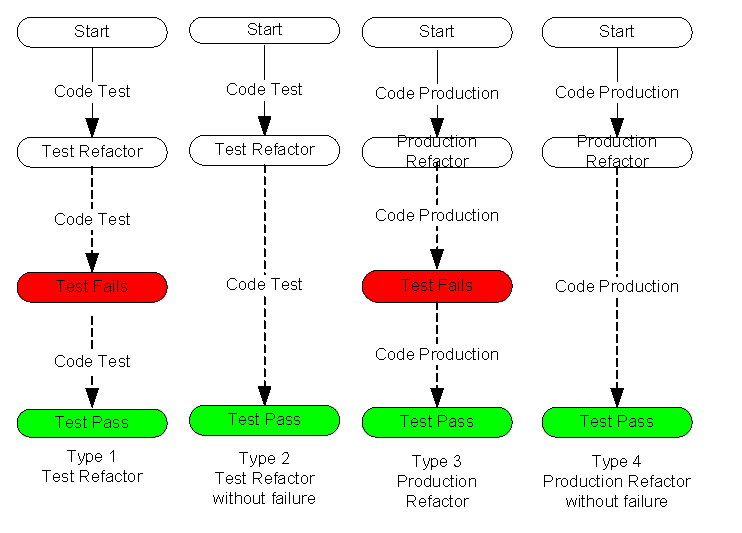
\includegraphics[width=0.8\textwidth]{figs/Refactoring.eps}
  \caption{Refactoring Episode Classification}\label{fig:refactoring}
\end{figure} 

 as in Figure \ref{fig:EpisodeTree}.
\begin{figure}[htbp] 
  \centering
  \includegraphics[width=0.8\textwidth]{figs/EpisodeTree.eps}
  \caption{Episode Tree}\label{fig:EpisodeTree}
\end{figure} 

Some empirical case studies \cite{George:03}, \cite{Maximilien:03}
reported successes on TDD practice. According to these studies TDD group
passed more black box tests than TLD group and they spent less time on
projects than TLD group. Even though most empirical studies drew positive
conclusion on Test-Driven Development there are still some neutral or
negative reports on TDD. Geras etc. \cite{Geras:04} found that there is
little or no difference in developer productivity in TDD and TLD processes.
Another study \cite{Muller:02} concluded that TDD does not accelerate the
implementation and the resulting programs are not more reliable than TLD.

\section{Validation}
Unlike many other cumbersome software processes such as Spiral model, PSP or
RUP Test-Driven Development is very lightweight. It contains two simple
rules only. In practice TDD is hard to follow compared to other processes
because there is no management involved in the development. In situations
that pair programming is not involved developers are fully responsible for
TDD execution by themselves without monitoring. This weakness will bring
many questions to TDD process. Do developers do Test-Driven Development
when they are told to do so? And if they do how well they do TDD in their
development? Do developers always follow two TDD rules?

In my thesis study I will build a system on top of Hackystat to answer
these questions as well as provide a tool to discipline TDD process.  There
are two goals to pursue in my work. One is to study how the development is
being done, especially how the unit testing is conducted in Test-Driven
Development. Another goal is to study properties of TDD. Will developers
spend more time on development and yield high quality code or not? Will the
test coverage be naturally 100\%?

Scott Ambler's UML diagram (Figure \ref{fig:TDDSteps}) depicts TDD development
iterations.

\begin{figure}[htbp] 
  \centering
  \includegraphics{figs/TDDSteps.eps}
  \caption{The Steps of TDD}\label{fig:TDDSteps}
\end{figure} 

\begin{itemize}
\item The first step is to add a test quickly. Basically it just fails the
  code.
\item Next run your test or test suite to make sure the new test does fail.
\item Make changes to the function code to make test pass. As long as it
  can make test pass you even can fake the implementation, for instance,
  return a constant number.
\item Run your tests again. If it still fails you go ahead to update your
  function code. Once all tests pass you can start over with a new test.
\end{itemize}

In the early era of software development there is no software process.
Software systems are developed in a chaotic style and their successes
depended largely on individual's skills and capabilities. Water-fall model
is the first and most popular software development process and it still
exists in many organizations. In water-fall model software development is
divided into stages from requirement analysis to operation and testing is
conducted after project is implemented. Bugs and defects found in testing
will be fed back to the development team or maintenance team. Since bugs
and defects are revealed at the late stage of software development
water-fall model is reluctant to meet customer's requirements and defect
fix. If defects are rooted from design it will be extremely hard to adapt
changes according to water-fall model.

Modern iterative incremental development(IID) was developed to fix this
problem by dividing a large project into many parts.  They are implemented
iteratively. Each iteration can be a mini-waterfall process so that defects
can be fixed and changes can be made very quickly.  Spiral model is the
first process definition to formulate iterative incremental development
practice. Other variations like prototyping, RAD, CleanRoom, Scrum, RUP,
FDD, Extreme Programming are used in many projects successfully.  Latest
development of continuous integration builds system once a day. In these
processes testing is done after some amount of work is finished to improve
project quality.
  
\section{Personal Software Process}
\label{sec:psp}

   Introduce LEAP and Hackystat.

\section{Test-Driven Development}
\label{sec:tdd}

\subsection{Unit Testing}
\label{sec:UnitTest}
Object-oriented technique treats abstract concepts as entities such that
each of them is independent and can exist without relying on other code.
Unit testing was invented to test a component before it is integrated to
interact with other components. Unit testing originates from
pre-object-oriented era and an individual test concentrates on a single
unit of the system rather than on the entire system. At present when we say
unit testing it refers to component testing. In object-oriented world a
component test usually tests an object or class which is the smallest component
of a system. ``In computer programming, a unit test is a method of testing the
correctness of a particular module of source code.'' \cite{UnitTestWiki}

Unit testing is becoming more and more popular in modern software
development.  The de facto unit testing standard, ``xUnit'' framework, is
already ported to more than 30 language support. It makes test automation
be feasible and test cases created with XUnit framework can server as
regression test suite too. Except for verifying correctness of each class
unit testing is also the executing documentation. In recent software
project development unit testing is integrated into development process in
many organizations. Test cases are written by developers who are also
responsible for programs. Even though source code is visible to developers
but unit testing is still thought as black-box testing because it simulates
calls from other components.  

JUnit is the most well-known XUnit framework implementation in software
development and other dialects NUnit, CPPUnit, PyUnit so on and so forth
are created to make writing unit tests be very simple in different
programming languages. JUnit and NUnit also have IDE plug-in supports so
that a unit test case can be exercised by just a single click. For
continuous integration unit test cases can also be batched together to run
as ANT task. Since writing unit tests is not a cumbersome job any more it
is recommended to write unit tests in the development process instead of
allocating extra resource to let quality assurance testers to create unit
tests separately. It improves the effectiveness of testing such that
software systems are in high quality before they are delivered to quality
assurance department or customers if there is no quality assurance process.
Since less time is needed to do quality assurance it will save overall
development time conceptually.


In TDD unit testing is crucial because it drives the implementation and provides
instant feedback of the developing code to the developers. The XUnit
framework family make it easy to write tests and execute tests often in
software development.

\section{Thesis Work}

\section{Road Map}

\label{sec:ResearchObjective}
Test-Driven Development is being accepted by more and more developers and
organizations. On the other side there are still many developers and
researchers resist Test-Driven Development or doubt its effectiveness in
software development. Kent Beck argued that TDD will not increase
development cost but can actually improve productivity as well as software
quality. Ron Jeffries's pithy word ``Clean code that works'' is the goal
of Test-Driven Development.


\section{Extreme Programming(XP) and Test-Driven Development(TDD)}
[How good is unit test? and why TDD]

This testing pyramid corresponds to software system development process.
In general a large system is divided into many components to be implemented
independently. Unit testing is created to verify correctness of each
component before it is integrated into the system.
  
Usually unit testing is done by programmers themselves to verify the
correctness or by quality assurance specialists to find errors in the
existing code.  According to the cost model of removing bugs in different
software development stages removing bugs in development phase is the most
cost-effective way.  Because unit testing is good from many aspects Extreme
Programming, an agile software development process, advocates Test-Driven
Development (TDD) as its core component. In TDD unit tests are
incrementally written prior to code implementation \cite{George:03} thus
it drives software specification design in addition to validating and
verifying program correctness. Because of this capability TDD is also
called Test-First Design (TFD). As comparison the old way writing unit
tests after code is ready is called Test-Last Development(TLD).
  
  
  The controversial conclusions can be either from TDD process itself or
  from the poorly executed experiments. There is one thing in common that
  all these studies failed to address how they managed experiments to
  guarantee TDD developers do Test-Driven Development while TLD developers
  do Test-Last Development in their studies. There is no process data
  available to crossly validate process disciplines. The lack of
  fine-grained process data and software metrics makes it impossible to
  conclude whether developers were doing TFD, ad-hoc or TLD in the previous
  experiments; thus, conclusions drawn from these experiments are weakened
  and become questionable. In my thesis I will add in-process metric
  support provided by Hackystat to study how unit tests are created and
  exercised in the development process to regulate software development.
\section{Testing}
\label{sec:Testing}
Testing is very important to software project success because developers
can not always produce perfect code that works well at the first time. Many
reasons determine that we need testing in software development. First of
all, many software systems deal with large number of states with complex
algorithms, also it is hard and impossible to address all system
requirements at the beginning of software projects development. Developers
always have to deal with new and changing requirements during the
development.  Another important factor is that software projects are
written by developers.  As human beings developers are not good at
repeative programming work without committing mistakes.  Since software
development is error-prone many design and development support tools such
as flowchart, dash board, UML , compilers, debuggers, version control
system, project management software, bug tracking system and software
review etc are brought up to support qualitative software development.
Moreover, there are rare software projects developed and maintained by an
individual programmer nowadays. The ineffective collaboration and
cooperation in the developing team will make software volatile to defects
and bugs too \cite{Pfleeger:01}.  To ensure software quality there are
quality assurance departments in many software institutes and many testing
techniques appeared in the development of software engineering discipline.
From visibility of source code there are white-box testing and black-box
testing. Depending on when testing happens there are unit testing,
regression testing, integration testing, system testing and acceptance
testing which can be done by programmers, quality assurance testers or
customers manually or automatically.

\begin{figure}[ht] 
  \centering
  \includegraphics[width=0.5\textwidth]{figs/TestLayerPyramid.eps}
  \caption{Software Testing Pyramid}\label{fig:TestLayer}
\end{figure} 

In tradition, software testing is thought as quality assurance testers' or
customers' job in water-fall software process model. Even in recent
iterative incremental development (IID) models quality assurance
specialties and customers still play important roles on testing.


\section{Software Processes}
\label{sec:SoftwareProcess}
In the early era of software development there is no software process.
Software systems are developed in a chaotic style and their successes
depended largely on individual's skills and capabilities. Water-fall model
is the first and most popular software development process and it still
exists in many organizations. In water-fall model software development is
divided into stages from requirement analysis to operation and testing is
conducted after project is implemented. Bugs and defects found in testing
will be fed back to the development team or maintenance team. Since bugs
and defects are revealed at the late stage of software development
water-fall model is reluctant to meet customer's requirements and defect
fix. If defects are rooted from design it will be extremely hard to adapt
changes according to water-fall model.

Modern iterative incremental development(IID) was developed to fix this
problem by dividing a large project into many parts.  They are implemented
iteratively. Each iteration can be a mini-waterfall process so that defects
can be fixed and changes can be made very quickly.  Spiral model is the
first process definition to formulate iterative incremental development
practice. Other variations like prototyping, RAD, CleanRoom, Scrum, RUP,
FDD, Extreme Programming are used in many projects successfully.  Latest
development of continuous integration builds system once a day. In these
processes testing is done after some amount of work is finished to improve
project quality.



\section{Extreme Programming}
\label{sec:XP}
Extreme programming (XP) grows very fast recently and many organizations
are using it or considering to adopt it in their developments. Extreme
Programming is also one kind of iterative incremental development (IID)
process.  It begins with collecting ``user stories'', which are brief
description of tasks to be accomplished. Developers can discuss with on-site
customers to make release plan based on user stories. After each release
customer can test the sub system and give feedback to developers quickly.
XP can not only meet customers' changing requirements well but also provide
high quality code because it stresses heavily on unit tests in the
development. Four rules are enforced in extreme programming.

\begin{itemize}
\item All code must have unit tests.
\item All code must pass all unit tests before it can be released.
\item When a bug is found tests are created.
\item Acceptance tests are run often and the score is published.
\end{itemize}

To enact these rules XP projects should be developed in Test-Driven
Development process, in which unit tests are created before code
implementation.  Developers write unit tests based on user stories first
and then generate code to make test pass.
\end{comment}



















\chapter{Related Work}
\label{chap:RelatedWork}

\section{Extreme Programming and Test-Driven Development}
\subsection{Extreme Programming}
Extreme Programming (XP) is a light-weight methodology for
small-to-medium-sized teams developing software in the face of vague or
rapidly changing requirements \cite{Beck:00}. It take common-sense
principles and practices to extreme level.
\begin{itemize}
\item If code reviews are good, we'll review code all the time (Pair Programming). 
\item If testing is good, everybody will test all the time (unit testing),
  even the customers (Functional Testing).
\item If design is good, we will make it part of everybody's daily business
  (Refactoring).
\item If simplicity is good, we will always leave the system with the
  simplest design that supports its current functionality (the simplest
  thing that could possibly work).
\item If architecture is important, everybody will work defining and
  refining the architecture all the time (Metaphor).
\item If integration testing is good, then we will integrate and test
  several times a day (Continuous Integration).
\item If short iterations are good, we will make the iteration really,
  really short--seconds and minutes and hours, not weeks and months and
  years (Planning Game).
\end{itemize}

XP is an agile process including 12 practices of: Planning Game, Small
Releases, Metaphor, Simple Design, Testing, Refactoring, Pair Programming,
Collective Code Ownership, Continuous Integration, Forty-hour Week,
On-site Customer and Coding Standards. \cite{Beck:00} As Kent Beck said XP is
not from ground up but many good practices derived from previous software
development. In XP these 12 practices support each other and complement
each other's weakness.  (Figure \ref{fig:XPSupportNetwork} Excerpted from
P70 \cite{Beck:00})
\begin{figure}[ht] 
  \centering
  \includegraphics[width=0.8\textwidth]{figs/XPSupportNetwork.eps}
  \caption{XP Support Network}\label{fig:XPSupportNetwork}
\end{figure} 

A typical XP project starts from planning game. Release plans will be laid
out in the planning game. Each release will vary from several weeks to
several months but not over half a year. Customers or stake holders define
release scope and important or critical business components go first.
Because XP is aiming at building simple but works software the advanced and
not-necessary features will not be considered until demanded. This will
maximize the Return-on-Investment (ROI). Communication, simplicity,
feedback and courage are four values XP will provide. Communications between
customer and developer, coach and developer, inter-developers are
encouraged by XP practices such as on-site customer, metaphor, coding
standard, collective ownership and pair programming directly or indirectly.
Feedback and courage are provided by test-driven development, on-site
customer, pair programming and continuous integration.  Simplicity is the
theme of XP through the entire development.  XP is another kind of
iterative incremental development (IID). The release plan is iterative and
development in each release is iterative too. Iteration in development is
from user story that can last only several days. The task assignment is
done in stand-up meeting. \cite{Beck:00}

Management of XP is through metrics, coaching, tracking and intervention.
It has roles developers, customer, tester, tracker, coach, consultant and
big boss. These roles are responsible for smooth execution and balance
maintenance of all 12 XP practices. Though XP acknowledges that each
practice has its own weakness it is not feasible for a developing team to
tranfer to XP seamlessly. Don Wells \cite{Beck:00} commented that XP
adoption can be iterative:
\begin{enumerate}
\item Pick your worst problem.
\item Solve it in XP way.
\item When it is no longer your worst problem, repeat.
\end{enumerate}

As we already know XP consists of 12 practices. Many of them can exist
independently. Planning game can fit into other IID process. On-site
customer can be available to other process models such as water-fall model.
Among 12 XP practices Pair Programming (PP) and Test-Driven Development
(TDD) often exist independently. They are widely applied and studied by
software developers, educators and researchers.

\subsection{Pair Programming}
Pair programming is an Extreme Programming practice. In pair programming
two programmers sit side-by-side at one computer, continuously
collaborating on same design, algorithm, code or tests. One acts as the
driver who types at computer. Another one acts as the navigator who is
responsible for high-level tasks like over-viewing design strategy,
inspecting code being typed for typos, syntax errors, or defects. Roles in
pair programming are dynamic and they can be exchanged during the
programming session or rotated in different programming sessions. Also the
pairs can be dynamically formed in a developing team. Two people actively
work on the same programming task with continuous collaboration.

Pair programming takes the privilege of code inspection a.k.a. code review
to improve code quality. Even though design or coding errors still can
exist but they will not last long because driver has to explain what he or
she is doing to navigator which provides a chance for both parties to think
it over. It looks like resources are wasted in pair programming because two
developers are invested on tasks that can be done by a solo developer;
however, Laurie Williams's case study concluded that pair programming will
not double development effort. In her study paired programmers are only
15\% slower than two independent individual programmers but produced 15\%
fewer bugs.  The knowing fact is that test and debug cost will be much
higher than initial programming so it will be economically paid off,
especially when some team members have to leave.

In extreme programming pair programming serves multiple purpose. Programs
are written by driver and navigator such that code review is done
simultaneously. The duo continuously communicate for better solution and
everyone inspects other's work. If driver goes the wrong way it can be
adjusted quickly by navigator without committing more mistakes, for
instance, when driver is not creating a test case before implementation
navigator can point it out so that they stay on the right track. Since
driver and navigator are exchanged during development both parties know
code well and own it. In case one programmer has to leave the developing
team risk is minimized because other people can take his or her work
over easily. The other benefit of pair programming is that junior
programmer can be coached and knowledge can spread over in the
team.\cite{PPWiki}

\subsection{Test-Driven Development}
Test-Driven Development is another Extreme Programming practice that has
its own benefits alone like pair programming. It's both the developing
method and design tool in extreme programming. Often it is called
Test-First Design (TFD) or Test-First Programming (TFP) because of its
natures. It has two fundamental rules:
\begin{itemize}
\item Write new code only if an automated test has failed.
\item Eliminate duplication.
\end{itemize}

Development of TDD is iterative. Test and implementation are added
incrementally under these two rules. An iteration can be elaborated as
following \cite{TDDWiki}:

\begin{enumerate}
\item Write the test
\item Write the code
\item Run the automated tests
\item Refactor
\item Repeat
\end{enumerate}

TDD is on the ground of a universally agreed claim that testing is good
to software project success. If it is done perfectly there is no need to
have a coverage tool because system is always 100\% tested. It supports
simplicity since developers only need to write enough code to make test
pass. Refactoring happens at the end of each iteration. Also unit tests can
serve as executing documentation of system so that re-usability is
improved.

In TDD unit tests are supported by XUnit framework. It is brought up by
Kent Beck, Ward Cunningham and Ron Jeffries in 1996 \cite{XP96}. It has the
following structure \cite{Beck:03}:

\begin{enumerate}
\item Invoke test method
\item Invoke setUp first
\item Invoke tearDown afterward
\item Invoke tearDown even if the test method fails
\item Run multiple tests
\item Report collected results
\end{enumerate}

In recent years xUnit has already been ported to more than 30 language
supports such as JUnit for Java, PyUnit for Python, NUnit for C\#.NET,
PHPUnit for PHP, CPPUnit for C++, DUnit for Delphi etc. \cite{XPSoftware}
and it has becoming the de facto standard of unit testing in software
development. With xUnit the unit testing is shifted from quality assurance
specialists or customers to developers.

This framework modulates unit testing onto method level. All public methods
in object-oriented domain are testable with this framework. It moves unit
testing from customer-oriented functional testing to the combination of
developer-oriented unit testing and customer-oriented functional testing.
Once project is brought up for functional testing it is already in high
quality insured by unit testing.

Theoretically speaking it is possible to do TDD perfectly but it is not
feasible in reality. First, developers as human beings are not good at
executing these two rigid rules. Second, there exists many holes such that
it is either not possible to do unit testing to some code or practically
infeasible in some cases. For instance, private methods are not accessible
for test purpose unless developer exposes them; GUI or event-driven methods
are not testable because they need humans intervention to make it happen;
some operations like database accesses are very time consuming such that unit
testing will take long time to run. Because of these limitations developers
would  not be able to follow TDD rules perfectly as Kent Beck wished.

In extreme programming process TDD can be executed better because other
practices can support it as figure \ref{fig:XPSupportNetwork} shows. Pair
programming supports TDD because two brains are better on creating good
unit tests and navigator can inform driver if unit tests are not created
before implementation. Coach can help pairs to design unit testing in case
it is hard or infeasible to do unit testing. Continuous integration can
help developers be aware of some unit tests fail or there is no unit test
to some code.


\section{Test-Driven Development in Practice}
Test-Driven Development is an incremental software development methodology
that stresses on exhausitive unit testing by creating test cases before
code implementation. It's a design and implementation methodology but
testing.  It ends with a rich suite unit test cases and high quality code
as it promises. It appears very often in software development tutorial
workshops
(\cite{OsheroveWorkshop:04,ClarkwareWorkshop:04,BENUGWorkshop:04,AdaptionTddWorkshop,IntustrialLogicTddWorkshop}),
technical reports, journals (\cite{TestDrivenDotComArticles}) and
blogsphere (\cite{TestDrivenDotComWeblogs}). Also many commercial and
open-source supporting tools (\cite{TestDrivenDotComTools}) are developed
in recent years.

\subsection{Characteristics of Test-Driven Development}

\subsubsection{Disciplined Small Steps}
In TDD development is incremental and iterative. Developers only write a
small portion of a unit test, or just one assertation each time, and then
just write enough code to test pass. At the beginnig the test target does
not exist so it cannot pass compilation. For instance, before we create
class Stack for a stack implementation we create a test class called TestStack.

    \begin{verbatim}
    package com.stack;

    import junit.framework.TestCase;

    /**
     * Tests stack operations. 
     */
    public class TestStack extends TestCase {
    }
    \end{verbatim}

To test whether stack can report its emptiness correctly developer adds one
assertation only in the first iteration.

    \begin{verbatim}
      /**
       * Tests empty stack.
       */
      public void testEmptyStack() {
        Stack stack = new Stack();
        assertTrue("Test empty stack", stack.isEmpty());
      }
    \end{verbatim}

It is not runnable because Stack class is not created yet. After creates
dummy implementation or stub of Stack it still cannot be compiled because
isEmpty() is not provided.

    \begin{verbatim}
    package com.stack;

    /**
     * Implements a stack.
     */
    public class Stack {
      /**
       * Constructs a stack.
       */
      public Stack() {
      }
    }
    \end{verbatim}

To make it compile developer goes ahead to add method isEmpty() which just
returns a constant.
    \begin{verbatim}
      /**
       * Whether stack is empty.
       * 
       * @return True if stack is empty.
       */
       public boolean isEmpty() {
         return false;
       }
    \end{verbatim}

Now it compiles but test fails because isEmpty() method simply returns
false. To make test pass developer changes it to return true. Then he/she
can go ahead to add another assertation and test case. As we can see from
above example development pace is really small in TDD. Generally one
iteration or cycle lasts from 30 minutes to 5 minutes. It rarely grows to
10 minutes \cite{GaryPollice:03}. It is totally okay to just add
implementation stub or simply returns a constant value to fake 
implementation (p13 \cite{Beck:03}, p169 \cite{Astels:03}).

\subsubsection{Consistent Refactoring}
Refactoring is an important portion in Test-Driven Development, it the
second TDD rule. By definition, refactoring is a disciplined technique for
restructing an existing body of code, altering its internal structure
without changing its external behavior \cite{Refactoring}. To make it
simple and concise refactoring is to change a program's interal structure
without affecting its external behaviors. In TDD developers need to
consistently do refactoring to support growing test suite without leaving
implementation code badly structured. When we do TDD the first priority is
to get test pass and the next is to remove duplication \cite{Beck:03}.
These two steps fulfil a complete TDD cycle. "Make it run, make it right.''
p24 \cite{Beck:03} Using the above example we can refactor isEmpty()
method to return an instance variable instead of a constant.
    \begin{verbatim}
      private int size = 0;
      /**
       * Whether stack is empty.
       * 
       * @return True if stack is empty.
       */
       public boolean isEmpty() {
         return this.size == 0;
       }
    \end{verbatim}

Now we run TestStack it passes. The duplication can be either on test code
or production code. As long as you get all tests pass you are confident to
do refactoring because unit tests can ensure you will not commit
unrecoverable big mistake.

\subsubsection{Courage, Rapid Feeback and One Ball in the Air at Once}
Kent Beck thinks TDD is a way of managing fear during development
\cite{Beck:03}. Programmers are in fear in software development because the
requirements are not clearly stated, techniques are new, problems are hard
to solve, or there is no enough time to do a thorough design and review.
Fears happen more often to novice programmers but experienced programmers
have fears too because a smallest mistake may break the whole system.
Experience programmers are good at debugging and have better intuition on
finding and solving bugs than novice programmers. In TDD developers ``test
a little, code a little and repeat.''\cite{Beck:03} Test cases guard code
development and provide instant feedback. Since the incremental step is
small it is impossible to commit big mistakes. If test fails it is easy to
fix it too. In software development developers carry the baggage with
requirement, system structure design, algorithm, code efficiency,
readibility and communication with other code etc. According to Martin
Fowler it is like keeping several balls in the air at once (Page 215
\cite{Beck:03}).  In TDD you only keep one ball in the air at once and
concentrate on that ball properly. Developer only needs to make the test
pass without worrying it is a good or bad design in TDD. In refactoring
step developer only worries about what makes a good design. Keeping one
ball only in the air helps doing good job on every aspect.

\subsubsection{Always Working Code}
TDD developers maintain a comprehend unit test suite and all test pass at
the end of each TDD cycle. The developing system is always working to the
designated tasks represented by unit tests. Since all test cases are
created in the domain of xUnit framework they can be integrated together to
do continuous integration. A test bot or agent can be setup to run all
tests everyday or every few hours \cite{ContinuousIntegration}. It works
well especially in team software development or in case it is not feasible
for a developer to run all tests in development in time manner.

\subsection{Benefits of Test-Driven Development}
\subsubsection{100\% Code Coverage}
If it is done perfectly TDD should always yield 100\% code coverage
\cite{Beck:03,Jeffries:00} as figure \ref{fig:TestScores} shows (Excerpted
from page 139 \cite{Jeffries:00}).
 
\begin{figure}[ht] 
  \centering
  \includegraphics[width=0.8\textwidth]{figs/TestScores.eps}
  \caption{Unit Test Scores}\label{fig:TestScores}
\end{figure} 

In practical it is not feasible to maintain 100\% but TDD developers do
yield high code coverage. Boby George and Laurie Williams's study finds
that TDD developers' test cases achieved 98\% method, 92\% statement and
97\% branch coverage \cite{George:02}. The experiment was conducted on a XP
developing team with Pair Programming practice too. Another study conducted
by Matthias M\"uller and Oliver Hagner in University of Karlsruhe found
that TDD developers yielded 74\% median branch coverage \cite{Muller:02}.
It's quite surprising because it is even lower than control group without
doing TDD whose median coverage is 80\%. On the fact that it is impossible
or not necessary to achieve 100\% this test coverage is still low. 

\subsubsection{Regression Test}
One principle of TDD is to create a regression unit test if system breaks.
The test fails first just as a typical TDD iteration. Code isolation is
another TDD principal that reduces coupling between objects. High CBO is
bad in object-oriented programming from modular design and reuse point of
views \cite{CKMetrics}. It's also straight forward the coupling can not be
zero because differant parts have to interact to make the system work. In
TDD developers run all tests regressively to make sure the new change will
not break other parts. Speaking in Java all package should have class
\verb!TestAll!  which assemblies all unit tests in the same package
together. When developer is working she or she just focus on tests in this
small area. XP has another practice called continuous integration to
execute all unit tests in timely manner to check system's consistency. If
the new change breaks system developer will know it in a few hours or a
day. A byproduct of TDD is a very comprehensive and exhaustive test set
that can serve as regression test suite.
 
\subsubsection{Executable Documentation}
In TDD there is no stacked written design documentations instead of
executing design documentation in unit tests. They are system-level
documentation and show how developers intended for the class to be used
\cite{ObjectMentorTDD,Ambler:03}.

\subsubsection{Clear Design}
XP community argues that TDD is not about test but design \cite{North:01}.
There is no big up-front design in XP and TDD but small incremental change.
Design decision is made incrementally by refactoring. Developers do
incremental change to the current code base instead of following design
documentation. Jim Little concluded that this evolutionary design yields
better results than big up-front design \cite{Little:01}. The design
architecture with upfront design generated a five-layer structure for data
persistence which is too complex in practice and the developing team was
completely lost. Intead the evolutionary is easy and effective in
architecture design. Also, TDD developer will not do anything extra except
for passing unit tests. It makes clean code that works \cite{Beck:03} and
is testable.

\subsubsection{High Quality Code}
Probably the most significant benefit of TDD to software development is
high code quality. Generally speaking TDD developers write code with high
coverage and the software created with TDD is more reliable than non-TDD
approach. Matthias M\"uller and Oliver Hagner's experiment in University of
Karlsruhe found that Test First Group (TFG)'s program has higher reliabilty
than controll group's code. In their experiment five TDD developers achieve
reliability over 96\% compared to only one program from the control group
that achieved this\cite{Muller:02}. Using black box test as external
validation TDD pairs passed approximately 18\% more black box tests in case
study conducted by Boby George and Laurie Williams \cite{George:03}.

\subsubsection{Increased Productivity}
TDD is faster test-last and code-N-fix. In TDD, testing is part of the
design process, it doesn't take long time to write a small test
\cite{MemoRandaBlog}. It is faster than test-last because developers need
to spend same amount or more time on creating tests after implementation.
Boby George and Laurie William's study showed that TDD developer spent 16\%
more than controller group but controller group did not primarily write any
worthwhile automated test cases though there were instructed to do so. TDD
code is much more reliable and with high code coverage. Since code is less
buggy it will save a lot time on debugging and maintenace.
\begin{quote}
``I have spent enough time in my career on silly bug-hunting, with TDD those
days are gone. Yes, there are still bugs, but they are fewer and far less
critical'' -- Thomas Eyde \cite{ExtremeJSBlog}
\end{quote}

\subsection{Barriers of Test-Driven Development}
More and more developers turn to TDD and many comercial and free workshops
are provided to evangelize TDD
\cite{TestDrivenDotComWeblogs,TestDrivenDotComArticle}.  Also, many tools
are created to support TDD \cite{TestDrivenDotComTools}. But still, many
developers are reluctant to TDD or even to give it a serious try despite on
the claim that TDD is infective \cite{Beck:03,TestInfected,EichertBlog,MasonBlog}. 
\subsubsection{Testability}
Darach Ennis argued that there are a lot of fallacies blowing around
various engineering organization and among various engineers \cite{Beck:03}. 
\begin{quote}
\begin{itemize}
\item You can't test GUIs automatically (e.g. Swing, CGI, JSP/Servlets/Struts)
\item You can't unit test distributed objects utomatically (e.g., RPC and Messaging style, or CORBA/EJB and JMS)
\item You can't test-first develop your database schema (e.g. JDBC)
\item There is no need to test third party code or code generated by external tools
\item You can't test first develop a language compiler/interpreter from BNF
  to production quality implementation.
\end{itemize}
\end{quote}

Most of these arguments are still valid but some operations are testable
nowadays. JSP and servlets can be tested by HttpUnit\cite{HttpUnit} or
Cactus\cite{Cactus}.  Mock object and Easy Mock can be used to test some
complex operations by providing fake implemention to the real system
\cite{MockObject}.

\subsubsection{Too Much Tests}
TDD is about design. To implement a task or user story developer makes a
list of test cases and maintains it when code grows. When it is empty and
there is no more test case developers can think of, task is done. All code
comes with test and sometimes test code may be larger than production code.
Apparently developers need to spend time on tests which are not thought as
production from customer point of view. XP says that it saves money for
customers on debugging and maintance, which is still not proved yet. A
model about Return on Investment (ROI) of TDD was brought up by Matthias
M\"uller and Frank Padberg shows how TDD can pay off the investment on
test\cite{Muller:03}. So far there is still no case study on cost benefit
analysis on TDD yet.

\subsubsection{Small Steps and Time-Consuming}
In TDD developers make small step each time. There will have many context
swith between test code and production, also many IDE activities. Using
previous isEmpty() method as example.
    \begin{verbatim}
      /**
       * Whether stack is empty.
       * 
       * @return True if stack is empty.
       */
       public boolean isEmpty() {
         return false;
       }
    \end{verbatim}

It is such a trivial thing such that most developers can make it right
without having a failed test. Kent Beck's opinion is that you can write
test that encourages hundreds of lines of code and hours of refactoring but
the tendency of TDD is to have smaller steps over time. Some developers
switched to TDD when old method cannot work, on example is defect removing
in debug.

\subsection{Testing Techniques and Tools}
\subsubsection{XUnit and its Related Tools}
XUnit is the corner stone of TDD. It makes test very simple and test
automation possible. The variation of xUnit includes JUnit for
Java\cite{JUnit}, SUnit for Small Talk\cite{SUnit}, CPPUnit for
C++\cite{CPPUnit}, NUnit for C\#.NET\cite{NUnit}, VBUnit for
VB\cite{VBUnit}, PYUnit for Python\cite{PYUnit} etc.  There are also some
extention for JUnit to test some complex operation, for instance, HttpUnit
for web\cite{HttpUnit}, Cactus for Servlet\cite{Cactus}, and DBUnit for
database\cite{DBUnit}. A new test tool called TestNG is developed to
simplify unit test using annotation and configuration file \cite{TestNG}.

\subsubsection{Mock Object}

\section{Case Studies on Test-Driven Development}
E. Michael Maximilien and Laurie Williams assessed Test-Drive Development
at IBM in the development of a new IBM Retail Store Solutions
version.\cite{Maximilien:03} The initiation of TDD came from the fact that
defect rate of each revisions did not drop in Functional Verification Test
(FVT) though developers have rich domain knowledge. TDD was introduced to
the developing team to alleviate the recurrent quality and testing
problems.  In their study they found defect rate dropped by 50\% in FVT
whereas productivity was not affected.  They believe that the drop of
productivity by TDD was complemented by the adoption of Microsoft Project
Central project management tool. The byproduct of TDD is a substantial
suite of unit tests. They also made test automation be possible and tests
were exercised once a day with the integration support. They also verified
the moral of TDD -- "test-infected'' phrased by Erich Gamma\cite{Beck:03}.
Developers were positive on TDD and intended to continue using it in their
future development.

Boby George and Laurie Williams summarized their findings regarding to
Test-Driven Development in three trial experiments \cite{George:03}.  TDD
approaches yielded superior external code quality measured by a set of
black box tests. TDD developers' code passed 18\% more functional black box
tests than controlled groups' code. Their results also showed that TDD
developers took more time than controlled groups. Additionally controlled
group did not write worthwhile automated test cases, which makes the
comparison on productivity uneven. The projects created by TDD developers
have very high test coverage. The mean method coverage is 98\%, statement
coverage is 92\% and branch coverage is 97\%.

Another case study conducted by Matthias M. M\"uller and Oliver Hagner in
University of Karlstruhe to test development efficiency, resultant code
reliability and program understanding. They found that switching to TDD
does not improve productivity and the code will not be more reliable than
with TDD approach. The only improvement is on code reusability because
tests help developers to use method or interface correctly \cite{Muller:02}.

\section{Hackystat}
Hackystat is an in-process automated metric collection system designed and
built in Collaborative Software Development Laboratory in University of
Hawaii. The attached IDE and ANT build sensors can collect the development
activities including file editing, class creation, method addition and
deletion as well as software metrics like unit test invocations, build
invocations, dynamic object-oriented metrics and other metrics as well.
Using Hackystat rich software metrics can be collected automatically to
study the development process without much work effort involved.

\subsection{Software Metrics}
A software metric is a measure of some property of a piece of software or
its specification \cite{SoftwareMetricWiki:05}. Common software metrics
include source lines of code, object-oriented metrics such as number of
methods in a class, coupling between objects, number of children etc, and
other metrics like function points, bugs per thousand lines of code, code
coverage and so on. Software metrics are widely used in software process to
predict and manage software development. A famous word by Tom Demarco is
that you cannot control what you cannot measure in controlling software
development \cite{SoftwareMetricWiki:05}. Software metrics make software
development process be measurable and process improvement be feasible.  

Koch summarized that there are two sets of objectives of software metrics 
\cite{QPMetricsKoch} :
\begin{itemize}
\item Measures are needed to develop project estimates, to monitor progress
  and performance, and to determine if the software products are of
  acceptable quality.
\item To the software organizations measurement can be used to determine
  overall productivity and quality level, to identify performance trends,
  to better manage software portfolios, to justify investments in new
  technologies, and to help planning and managing the software function. 
\end{itemize}

\subsection{Personal Software Process}
Personal Software Process (PSP) is a manual approach to record personal
software development activities to help project planning and estimation.
It's created and evangelized by Watt Humphrey at Software Engineering
Institute (SEI) in Carneige Mellon University. SEI provides a series of
training courses for developers and educator to grasp it \cite{Humphrey99}.
PSP has four levels range from 0 to 3 and the training course provides 10
programming exercises and five reports. On level 0 developers learn to
record their current practice using time recording log to understand how
time is spent to improve time usage. Other metrics like project size and
defects are measured too on level 0. On level 1 developers will do project
planning and estimation with the metrics data collected to improve
estimation accuracy. Code review and design review are introduced on level
2 to improve personal software quality. Level 3 is called cyclic personal
process. It suggests developers should divide large tasks into small pieces
to develop with PSP as Iterative Incremental Development (IID) advocates.

Many researches and experiments were conducted on PSP. Most of them show
that developers can improve productivity and reduce defect density with PSP
and the estimation accuracy is improved. Some researches reported poor
support for team software development and issue with data collection. Ann
Disney found that data entry is error prone in PSP.

\subsection{Automated Personal Software Process}
PSP helps individual developer to improve personal software process
maturity. To lower data entry overhead and improve PSP data quality.
Carleton A. Moore developed LEAP Toolkit in Collaborative Software
Engineering Laboratory in University of Hawaii. With LEAP Toolkit
developers can record their time and enter data easily. It improves data
accuracy and provides regression analyses that cannot be done manually in
PSP \cite{csdl-99-15}.

\subsection{Hackystat}
Tools like LEAP Toolkits make it fairly easy to record PSP data and conduct
project planning and estimation. In LEAP developers enter PSP data using
clock control and other data entry forms but developers will have to stop
their on-hand work often to input data, which reduces its effectness on
process improvement, project planning and estimation. It is also hard to do
collaboration to support team project development. In 2001 Philip Johnson
etc started Hackystat project to collect development automatically.
Hackystat sensors can be installed in development environments such as
XEmacs, JBuilder, Eclipse and Visual Studio etc to collect software
development data unobtrusively. Hackystat sensors will send out metric data
collected to a centerized data server with SOAP protocol \cite{csdl2-04-05}
in a period-based fashion. Hackystat is extensible so that many kinds of
metrics can be collected except for time, size and defect measurement.
Most development activities such as opening file, editing file, closing
file and refactoring data can be collected by Hackystat sensors. Unit test
case exercises and test coverage can be recorded too by Hackystat. It
supports development collaboration by defining project with common
workspaces\cite{csdl2-04-05}. Initial case studies (\cite{csdl2-03-13},
\cite{csdl2-03-12}) found that Hacksytat has very low overhead for students
and Hackystat analyses are very helpful on student projects. Usage of
Hackystat on extreme programming, high performance computing, project
management and software reviews are being explored in Univeristy of Hawaii
and affiliate organizations.




















%\chapter{Implementation}
\label{chap:Implementation}

%%\begin{comment}
\section{Graphic View of Software Testing Process}
Software process is constructed by a series of analysis, design,
development, testing and debugging activities. It starts from requirement
analysis and ends after software products are delivered. Rational Unified
Process (RUP), Personal Software Process (PSP), Team Software Process (TSP)
and Extreme Programming (XP) are some well-defined software processes.
These processes were defined by process pioneers from their best practice
and critical thinkings on their development activities. All processes are
constructed by a set of rules and advices from requirement analyses to
testing. They exist in many kinds of software development organizations and
the rules are enforced by development team leaders or managers. Software
development process is thought as intellectual, non-repeatable and invisible.

In my thesis work I will focus on studying tests in software development,
especially Test-Driven Development to see how tests are being created and
exercised by developers incrementally. A test process view is going to be
implemented to display and analyze how developers create and execute tests
in their development. This tool is called TDPViewer, which stands for Test
Development Process Viewer. With this view support I will be able to
study development process to see whether developers follow a set of
demanded rules.
\section{Process Pattern and Quantification}
Speaking of unit testing execution in software development it could be
either test-first as specified by Test-Driven Development, test-last, or
hybid mode of test-first and test-last. In Hackystat we collect both the
development activities including implementation, compilation, unit testing
and debugging in Eclipse IDE so it is clearly feasible to study how unit
tests are implemented in the development process. Software process rules
can be used to generate development patterns to categorize how developers
do unit testing in the real implementation. One thought here is to design a
rule-based agent to study the development pattern [further research to be
conducted] to do the categorization.
%%\end{comment}





















\chapter{Zorro Case Studies}
\label{ch:evaluation}
Test-driven development is a low-level software process that consists of
many short-duration activites---file edit, compilation, unit test, debug, so
on and so forth. Zorro software system collects and analyzes on these
low-level and short-duration activites to detect the existance of
test-driven development with software development stream technology and
rule-based system supports. The test run and pilot study have demonstrated
that Zorro recognized test-driven development successfully. Yet,
following three issues are remained to be resolved before we deploy Zorro
in actual software development.
\begin{itemize}
\item \textit{Data collection problem:} Does Zorro collect fine enough
  developer behavioral data to recognize test-driven development?
\item \textit{Result correctness:} Does Zorro infer test-driven development
  correctly from the collected developer behavioral data?
\item \textit{Detection of alternatives:} Test-driven development is a new
  best practice and it may not be so perfect that it is applicable to all
  applications in all the time. Can Zorro tell the difference when
  developers do the alternative processes, such as test-last development
  --- developer writes unit tests afterward intead of test-driven?
\end{itemize}
Experiments and case studies should be carefully designed and carried on in
order to resolve these issues systematically. In January 2006, a pilot
validation study was conducted to test Zorro and the validating method,
which turned out to be a success\cite{csdl2-06-02}. Furthermore, an
expanded replication study is scheduled in a software engineering class in
fall 2006 for statistic correctness among junior TDD developers. According
to Yin \cite{Yin:03}, single case study in one organization suffers
external validity problem and research conclusions of it can not be
generally applied; therefore, I am going to conduct another case study with
experienced TDD developers. These three Zorro validation studies are
carefully designed and described in this chapter after an introduction of
Eclipse screen recorder utility\cite{esr}, a development process recording
tool.

\section{ESR: a tool for cross-validation}
\label{sec:esr}
To validate Zorro's data collection and TDD recognizing result, we should
have an independent and fine-grained data source on low-level development
activities for cross-validation. Considering that human being observation
of development process can not record fine enough activity data and video
recording with camcorder is too hassle to setup for test, I designed and
implemented ESR\cite{esr}, a lightweight development process recording
tool.

\subsection{Requirement analysis of ESR}
Zorro collects low-level development activities and infers test-driven
development process with the collected data. Compared to high-level process
activities such as requirement analysis and system design that may last
months or years, low-level development activities only last seconds or
minutes. Thus, one requirement is that ESR can record very fine-grained
data to observe activities happened in seconds.

Participants will send the software development process video recorded by
ESR to researchers for analysis via email. The video should be readable for
researchers to tell development activities from analysis wise, and size of
the videos must be small for transfer. 

Also, ESR can not use too much CPU resource while recording because
developers will develop software at the same time. In worst scenario, it
should not use more than 50\% CPU resource in order to avoid delay of
response for development activities.

\subsection{Design and implementation of ESR}
Participation observation and video recording are two most often used
approaches in human behavior related research. In the case of Zorro
validation study, participation observation is not plausible because human
being can not keep up the rapid pace of low-level software development
activities in short-duration. This leaves the alternative method, video
recording, as the only choice. Because laboratory test is expensive to set
up and it can deflect what developers normally do in their working
environment, we should allow them work in their familar environment. As the
trade-off, we ended up with a screen recording tool that can record changes
of computer screen caused by development activities.

The wide adoption of Eclipse IDE incites us to design and implement the
screen recording tool as an Eclipse plug-in named ESR\cite{esr}, acronym of
Eclipse Screen Recorder. It captures Eclipse screens in a fixed sampling
rate, computes delta changes of consecutive screens, and writes screen
changes into a movie file. Figure \ref{fig:esr-gui} is the ESR user
\begin{figure}[htbp] 
  \centering \includegraphics[width=0.6\textwidth]{figs/esr-gui.eps}
  \caption{ESR user interface}\label{fig:esr-gui}
\end{figure} 
\begin{figure}[htbp] 
  \centering
  \includegraphics[width=0.9\textwidth]{figs/esr-structure.eps}
  \caption{ESR Plug-in Structure}\label{fig:esr-plugin}
\end{figure} 
interface, which consists of a green button and a red button only in
Eclipse toolbar menu. Internally, ESR defines one abstract recorder and
three concrete recorder implementations using Java Media Framework, Flash
and Quick Time respectively as shown in figure \ref{fig:esr-plugin}.

\subsection{Using ESR}
We recommend QuickTime recorder because its video compressing rate is the
highest one among three ESR recorders: the size of one hour's software
development movie file typically ranges 5mb-10mb depending on main frame
changes and resolution preference. The only down side is that a fast
computer is desired for QuickTime recorder functioning well without causing
noticeable delay of response to software development activities in Eclipse
IDE.

ESR can be easily configured using Eclipse preference page as shown in
figure \ref{fig:esr-preference}.
\begin{figure}[htbp] 
  \centering
  \includegraphics[width=0.8\textwidth]{figs/esr-preference.eps}
  \caption{Configuration of ESR Plug-in}\label{fig:esr-preference}
\end{figure} 
Practical use of ESR found that it can capture 1280*1024 Eclipse window in
one frame per second rate, resize it to 960*680 image and create QuickTime
movie without significant lagging on a 2GHz PC.

\section{Pilot study}
\label{sec:pilot}
\subsection{Subjects}
\subsection{Experiment setting}
\subsection{Procedure}
\subsection{Data analysis}
\subsection{conclusion and discussion}

\section{Classroom study}
\label{sec:classroom}
The pilot study (Section \ref{sec:pilot}) proves that Zorro can collect
enough developer behavior data to derive test-driven development in high
accuracy, in the mean time it also confirms us that the validation study
procedure works well. To be statistically correct, we will conduct an
extended replication Zorro validation study in a software engineering class
in fall 2006.

\subsection{Goals and hypotheses}
As an extended study of pilot study on Zorro validation, the goal of this
study is to validate Zorro's capabilities on developer behavior data
collection and test-driven development recognition. Hypotheses to test are:
\begin{itemize}
\item{Hypothesis 1. }\textit{Zorro can collect enough developer behavior
    data to recognize test-driven development.}
\item{Hypothesis 2. }\textit{Zorro can correctly infer test-driven
    development with the collected developer behavior data.}
\item{Hypothesis 3. }\textit{Zorro can detect alternative processes when
    developers do not do test-driven development.}
\end{itemize}

Kent Beck, pioneer of test-driven development, ever claimed that developers
would be ``test infected'' after they give it a serious try. With the
capability of this study, we will evaluate this claim as well. The fouth
hypothesis is:
\begin{itemize}
\item {Hypothesis 4. } \textit{Students will get ``test infected'' and
    stick to tdd in their course projects development although test-driven
    development is elective.}
\end{itemize}

\subsection{Subjects}
Test subjects are students in a graduate level software engineering class.
Prior to the study we will ask students to sign consent form (see appendix
\ref{app:consent}) to inform them that this study is part of a scientific
research, data collected will not be used against their gradings and
participation is voluntary.  Human subject clearence exemption of this
reseach project was already granted by University of Hawaii Committee on
Human Studies.

\subsection{Experiment setting}
Elements of Zorro validation are Zorro-compliant IDE, Hackystat sensor for
developer behavior collection and ESR for development process recording.
Currently, only Eclipse IDE has a sensor that is designed to collect
development events suitable for Zorro processing. Hackystat Eclipse sensor
and ESR will be used to instrument students' test-driven development
process for colleting development data. In a nutshell, required experiment
settings are:
\begin{itemize}
\item \textit{Windows-based pc(\begin{math}\ge\end{math}1.8GHz CPU and
    \begin{math}\ge\end{math}512MB RAM})
\item \textit{JDK 1.4 or JDK 5}
\item \textit{Eclipse SDK 3.2}
\item \textit{Hackystat Eclipse Sensor (up-to-date version)}
\item \textit{ESR with QuickTime(up-to-date version)}
\end{itemize}

As discussioned in section \ref{sec:esr}, this experiment will not be
conducted in laboratory setting which may deflect how students write
program in actual situation. Instead, student participants will work on
their own PCs at the time to their conveniences.

\subsection{Experiment procedure}
Experiment procedure of this study includes four steps --- training,
practice of test-driven development, enactment of test-driven development,
and course project development in elective process.

\subsubsection{Training}
Software testing is a major topic of software engineering, but it used to
be taught by instructors in a later time as a software quality assurance
technique following the waterfall model. Modern software development
intends to emphasize on software testing at early stage of software process
to improve software quality. Thus, lectures on software testing will be
given at an early time in the software engineering class. Recommended
lectures are:
\begin{itemize}
\item {Lecture 1.} \textit{Software testing methods: system testing,
    validation testing, integration testing and unit testing. Reading
    materials: software testing chapter of textbook.}
\item {Lecture 2.} \textit{Methods and tools: xUnit, JUnit, JUnit in
    Eclipse, JUnit for ANT and Test-Driven Development. Reading materials:
    JUnit 3.8 Cookbook, preface and chapters 1-2 of book ``Test-Driven
    Development by Example''\cite{Beck:03}.}
\item {Lecture 3.} \textit{Software metrics, Hackystat infrastructure,
    software project telemetry. Assignment: install Hackystat sensor,
    develop some simple code, and invoke Hackystat analyses.}
\item {Lecture 4.} \textit{Test-Driven Development, Zorro software system,
    and Eclipse Screen Recorder. Assignment: install and configure ESR,
    develop a trivial problem in TDD with Eclipse sensor and ESR
    instrumentation.}
\end{itemize}

Consent form (appendix \ref{app:consent}) will be distributed to students
after we make sure that students can get along well with Hackystat and ESR.

\subsubsection{Practice of test-driven development}
It is needed and necessary to practice test-driven development for students
from a lesson learned in the pilot study: although test subjects were
explicitly told to do test-driven development with the supplied task list,
50\% episodes are neither test-driven nor refactoring in pilot study. In
addition, it is important to ensure that students are comfortable with
JUnit, test-driven development and instrumentation tools --- Eclipse sensor
and ESR. Therefore, we will ask students to practice test-driven
development on a well-known problem with the supplied tutorial chosen from
the following three candidates:
\begin{itemize}
\item Roman numeral converter: \textit{is a program that can convert any
    integer number between 1 and 50 to roman numeral.}
\item Stack: \textit{is a data structure that works in Last-In-First-Out
    principle.}
\item Bowling game: \textit{a single bowling game consists of ten frames.
    In each frame the object is to roll a ball at ten bowling pins.}
\end{itemize}

The practice of test-driven development will be instrumented by Hackystat
Eclipse sensor and ESR, and the collected data will be used to validate
Zorro. With this practice we will know that:
\begin{itemize}
\item \textit{students understand red/green/refactor rhythm of TDD with
    hands-on experience;}
\item \textit{students can get along well with ESR, the screen recording
    tool.}
\end{itemize}

A follow-up survey (see appendix \ref{app:pre-survey}) will be given to
students to investigate their opinions on test-driven development after
they finish the test-driven development assignment.

\subsubsection{Enactment of test-driven development}
In the previous step, students practice test-driven development on a well
defined problem with step-wise tutorial, which might be too easy compared
to actual problems in software development. Therefore, we will ask students
to work on their course projects using test-driven development for a while.
Purpose of this study is to: validate Zorro with actual software
development data; and urge students do test-driven development seriously.

Same as last step, students will develop software in Eclipse IDE with the
instrumentations of Hackystat Eclipse sensor and ESR. It required to do
more than 3 hours' test-driven development in the first week after course
projects are assigned. Development activity data and ESR video are
collected for Zorro validation analysis.

Another survey (apprendix \ref{app:post-survey}) will be conducted
thereafter to readdress student's opinions on test-driven development and
intention to continue using it in their future software development.

\subsubsection{Course project development in elective process}
In the rest of course project, we will no longer ask student to do
test-driven development and record development process with ESR. In turn,
students can choose any development method that works best for them and
their development process will be instrumented by Eclipse sensor only.

\subsection{Data analysis}
\subsubsection{Test-Driven Development recognition with Zorro}
Hackystat Eclipse sensor collects development activity data and send them
to Hackystat server automatically. A Hackystat project can be defined for
each student to recognize test-driven development with collected
development event data. Figure \ref{fig:zorro-gui} demonstrates Zorro
recognition results for project ``StackWithTDD''.
\begin{figure}[htbp]
  \centering
  \includegraphics[width=0.85\textwidth]{figs/zorro-interface.eps}
  \caption{Zorro Recognition Results}\label{fig:zorro-gui}
\end{figure} 
Zorro divides the software development stream into episodes and reports the
recognition results of episodes on left column in values---``tdd'',
``tld'', ``refactor'', or ``validation''. Developer behavior data drived
from development events and metrics for test-driven development inference
are displayed on the right column. Each activity includes timestamp when
the activity occurs, file that it is associated with, activity type, and
supplemental metric data.

\subsubsection{Development process video analysis}
In the development process video analysis, we will play the collected
videos with QuickTime player, write down the script of the development
process with a book keeping tool such as Microsoft Excel, and compare them
against development event data collected by Zorro for validation. Figure
\ref{fig:esr-video} is a screen copy of the
\begin{figure}[htbp]
  \centering
  \includegraphics[width=0.8\textwidth]{figs/esr-video.eps}
  \caption{Video of Development Process}\label{fig:esr-video}
\end{figure} 
development movies. The main screen is Eclipse window which records
development activities, and a time line track is attached to the movie at
the bottom for data synchronization. Table \ref{tab:video-narrate}
illustrates how we use Excel to do book keeping and Zorro validation.
\begin{table}[htbp]
\centering
  \caption{Zorro and ESR video comparison data sheet}\label{tab:video-narrate}
  \begin{tabular}{|l|l||l|l|l|l|p{3.5cm}|} \hline 
    \multicolumn{3}{|l}{Subject id: XXX-XX-XXX} & \multicolumn{4}{l|}{Movie file: esr-YYYY-mm-DD-hh-mm-ss.mov} \\ \hline\hline
    Episode \# & Zorro & Video & From & To & Activity & Annotation \\ \hline
    1 & (tdd, 1) & (tdd, 1) & 23:28:32 & 23:28:43 & New project & Create new project HelloWorld \\ \hline
          &          &          & 23:28:45 & 23:29:21 & New TestStack & Create unit test TestHello in package edu.hawaii.ics.rainer \\ \hline
          &          &          & 23:29:55 & 23:30:08 & Add testAloha & Add a empty test case for Hello \\ \hline
          &          &          & ...      & ...      & ... & ... \\\hline
          &          &          & 23:32:26 & 23:32:32 & Run TestHello & Test passes \\ \hline\hline
    2 & (tdd, 1) & (tld, 1) & ... & ... & ... & ... \\ \hline
          &          &          & ... & ... & ... & ... \\ \hline
  \end{tabular}

\end{table}
One by one comparison between bookkeeping data and Zorro developer behavior
data will give us insights whether Zorro data collection mechanism is
correct and whether the collected data are good enough to infer test-driven
development. A beauty of the video analysis is that it can give us insights
how software process is executed by developers, with which we can not only
validate Zorro but also find ways to improve it.

\subsubsection{``Test infected'' claim verification with telemetry}
Software telemetry \cite{csdl2-04-11} is a new approach of software project
management and telemetry report can give retrospective and in-process
analysis on software development process. Zorro defines three telemetry
reduction functions:
\begin{itemize}
\item \textit{MemberTestDriven} Computes Test-Driven Development percentage
  of a project member over the given time interval.
\item \textit{ProjectTestDriven} Computes Test-Driven Development
  percentage of a project over the given time interval.
\item \textit{ZorroEpisode} Reports number of episodes of a specific
  episode type, or total number of test-pass episodes over the given time
  interval.
\end{itemize}

By combining telemetry reports and students survey, we can verify whether
students get ``test-infected'' with strong evidences.

\subsection{Anticipated Results}
\begin{itemize}
\item Zorro collects development necessary behavior data correctly to
  derive test-driven development.
\item Zorro recognizes test-driven development in acceptable accuracy.
\item Students get ``test-infected'' and they continue using test-driven
  after Zorro validation study.
\end{itemize}

\section{Study in TDD community}
\label{sec:community}
Case study with students in classroom setting is insufficient for
generalization of conclusions as the matter of fact that students are
novice programmers and TDD developers. I plan to conduct an off-site case
study of Zorro by recruiting experienced TDD developers from test-driven
development community, the user group of TDD.

\subsection{Goals and hypotheses}
The objective of this study is to validate Zorro on developer behavior data
collection and test-driven development process recognition with experienced
TDD developers. Beyond this objective, I also aim at improving test-driven
development recognition capability of Zorro in actual software development
process. Propositions with regard to these goals are:
\begin{itemize}
\item{Hypothesis 1. }\textit{Zorro can collect enough developer behavior
    data to recognize test-driven development.}
\item{Hypothesis 2. }\textit{Zorro can correctly infer test-driven
    development with the collected developer behavior data.}
\item{Hypothesis 3. }\textit{Zorro helps experienced tdd developers stay on
    the track of test-driven development.}
\end{itemize}

\subsection{Subjects}
Test subjects are experienced TDD developers from the community of
test-driven development, user group of \cite{TddYahooGroup}. On the
account that I only have limited experience on recruiting
experienced/professional developers as test subjects, it will be wise to
take Benestad's advice \cite{Benestad}:
\begin{quote}
  first, practical constraints must be defined when defining the target
  population of software developers; second, participants must be offered
  flexibility and value using a planned communication strategy; third, high
  professional and ethical standard must be employed.
\end{quote} 
There principles are largely for recruiting professional developers from
software organizations for controlled experiments, but we can borrow the
idea to assist recruiting test-driven development community members who
likely belong to some software institutes.

\begin{enumerate}
\item \textit{Practical constraint must be defined when defining the
    target population of software developers.}\\
  The constraint is that participants must be okay with Java programming in
  Eclipse IDE in Windows OS. JUnit 3.8 is recommended.
\item \textit{Participants must be offered flexibility and value.}\\
  Test subjects have the flexibility to choose the problem to tackle in
  test-driven development to their conveniences. Process Instrumentation
  and data collection overhead are maintained in the lowest level. As the
  payback, participants can use Zorro in their organizations for
  test-driven development process improvement and I will provide technique
  support. Appendix \ref{app:letter} is the participation solicitation
  letter for recruiting experienced developers from test-driven development
  community.
\item \textit{High professional and ethical standard must be employed.}\\
  Clearence of human subject exemption was already granted by University of
  Hawaii Committee on Human Studies. Participants' individual skills will
  not be evaluated, instead their inputs will be used to evaluated Zorro
  software system. The participantion of this study is voluntary and test
  subjects can withdraw from the study at any time. A consent form
  (appendix \ref{app:consent2}) will be signed by participants and they can
  keep a copy of it for reference.
\end{enumerate}

\subsection{Experiment setting}
This study offers the flexibility to allow participants work off-site at
their own working environment. Basic requirements are:
\begin{itemize}
\item \textit{Windows-based pc(\begin{math}\ge\end{math}1.8GHz CPU and
    \begin{math}\ge\end{math}512MB RAM})
\item \textit{JDK 1.4 or above}
\item \textit{Eclipse}
\item \textit{JUnit 3.8}
\item \textit{Hackystat Eclipse Sensor}
\item \textit{Eclipse Screen Recorder}
\item \textit{Quick Time}
\end{itemize}
Java 5 features of JUnit 4.x are depressed for this study because Eclipse
sensor can not tell on-going metrics of Java 5 style code. In order to help
participants configure the test environment, we wrote a DocBook chapter for
reference in HTML at \cite{ZorroUserGuide}.

\subsection{Data collection}
The Java development in Eclipse IDE in test-driven development will be
instrumented by Hackystat Eclipse IDE and ESR. Once installed, Hackystat
Eclipse sensor can collect data unobtrusively. Developers start ESR
recording by pressing green button and stop it by pressing red button.
It takes test subject's manual intervention to send the recorded movie file
to reseachers for data analysis.

\subsection{Procedure}
\subsubsection{Recruition of test subjects}
A participation invitation email will be sent to test-driven development
user group to recruit test subjects. The first contact email will briefly
address objective of this study, introduction of Zorro software system and
what participants will do in the study. If some people are interested in
participation, I will send them consent form and instruction guideline for
the study.

\subsubsection{Test environment setup}
Participants will install Eclipse IDE if they've not done it yet, and
process instrumentation utilities --- Hackystat Eclipse sensor and Eclipse
screen recorder (ESR) under help of Zorro user guide\cite{ZorroUserGuide}.

\subsubsection{Development and data collection}
Developers can choose the problem they want to work on either from the
selected problem sets or elect their own software development in TDD.
\begin{itemize}
\item A well-known problem: stack, roman numeral or bowling game.
\item Another interested problem: money, sudoku, or spreadsheet.
\item 1-3 hours' personal software development in TDD.
\end{itemize}
The development process is instrumented by Hackystat Eclipse sensor and ESR
for data collections. Developers will send their recorded process video to
me using email for data analysis and answers to a short survey on usfulness
and usability of Zorro software system.

\subsection{Data analysis}
\subsubsection{Zorro validation analysis} 
We will be conducting similar analysis as in classroom case study
\ref{sec:classroom} to validate Zorro's data collection and TDD recognition
capability.

\subsubsection{Usefulness and usability of Zorro}
Feedback from experienced TDD developers is helpful on identifying issues
regarding to test-driven development discipline in practice and verifying
hypothesis 3 made on Zorro usefulness.





%\chapter{Time Line}
\label{sec:timelinel}

\begin{table}[ht]
\centering
\caption{Tentative Timeline}
\begin{tabular}{|c|c|} \hline
Task &  Milestone \\ \hline
Pilot Study of TDD and TLD & Jan 7, 05 \\ \hline
Development of TPDViewer & Feb 1, 05 \\ \hline
Form Committee & Feb 1, 05 \\ \hline
First Round TDD Experiment &  Mar 3, 05 \\ \hline
\#1 Survey on TDD Acceptance & Mar 4, 05 \\ \hline
Second Round TDD Experiment & Mar 20, 05 \\ \hline
\#2 Survey on TDD Acceptance & Mar 21, 05 \\ \hline
Third Round TDD Experiment & Apr 15, 05 \\ \hline
\#3 Survey on TDD Adoption & Apr 16, 05 \\ \hline
TDD Study on TDD Adoptors & Aug 8, 05\\ \hline
First Thesis Draft & Oct 10, 05 \\ \hline
Submit thesis to committee  & Nov 15, 04 \\ \hline
Thesis Defense & Dec 3  \\ \hline
\end{tabular}
\end{table}





















%\chapter{Conclusion and Discussion}
\label{chap:Conclusion}

\begin{comment}

%hongbing is cool.

To Be Done.

\end{comment}

\appendix
\chapter{Consent form of classroom case study}
\label{app:consent}
\noindent Thank you for agreeing to participate in our research on
understanding test-driven development practices. This research is being
conducted by Hongbing Kou as part of his Ph.D. research in Computer Science
under the supervision of Professor Philip Johnson.\\*[3mm]
As part of this research, you will be asked to develop or modify a program
and part of your course project using test-driven design practices and the
Eclipse development environment. While you are working on the program, we
will be collecting data about how you program, including the statements
that you write, the test cases that you develop, the times that you invoke
the tests and their outcomes, and so forth.  The development or
modification activity will typically take no more than a few hours of work,
depending upon how consistently you work on it.\\*[3mm]
There is no ``right'' or ``wrong'' way to do software development in this
research. Just develop the software as best you can. We are interested in
observing what real programmers do when working in a test-driven
development setting.\\*[3mm]
The data that we collect will be kept anonymously, and there will be no
identifying information about you in any analyses of this data.\\*[3mm]
Your participation is voluntary, and you may decide to stop participation
at any time, including after your data has been collected.  If you are
doing this task as part of a course, your participation or lack of
participation will not affect your grade.\\*[3mm]
If you have questions regarding this research, you may contact Professor
Philip Johnson, Department of Information and Computer Sciences, University
of Hawaii, 1680 East-West Road, Honolulu, HI 96822, 808-956-3489.  If you
have questions or concerns related to your treatment as a research subject,
you can contact the University of Hawaii Committee on Human Studies, 2540
Maile Way, Spalding Hall 253, University of Hawaii, Honolulu, HI 96822,
808-539-3955. \\*[3mm]
Please sign below to indicate that you have read and agreed to these
conditions.\\*[3mm]
Thanks very much! \\*[3mm]
----------------------------- \\
Your name/signature\\
Cc: A copy of this consent form will be provided to you to keep.


\chapter{Pre-survey on test-driven development}
\label{app:pre-survey}
\noindent Your email: \ldots\ldots\ldots\ldots\ldots\ldots\ldots\ldots\ldots\ldots\ldots\ldots\ldots\ldots\dots\ldots\ldots\ldots\\*[3mm]
Please circulate your answers to the following claims made on test-driven
development.\\*[3mm]
1. Test-driven development helps me develop code in less time: \\
(1) Strongly Disagree (2) Disagree (3) Neutral (4) Agree (5) Strongly Agree\\*[3mm]
2. Test-driven development drives me understand requirements and specification
better.\\
(1) Strongly Disagree (2) Disagree (3) Neutral (4) Agree (5) Strongly Agree\\*[3mm]
3. Test-driven development improves code quality. \\
(1) Strongly Disagree (2) Disagree (3) Neutral (4) Agree (5) Strongly Agree\\*[3mm]
4. Test-driven development helps to yield simple design.\\
(1) Strongly Disagree (2) Disagree (3) Neutral (4) Agree (5) Strongly Agree\\*[3mm]
5. Test-driven development saves time on debugging. \\
(1) Strongly Disagree (2) Disagree (3) Neutral (4) Agree (5) Strongly Agree\\*[3mm]
6. Test-driven development is more effective than other methods.\\
(1) Strongly Disagree (2) Disagree (3) Neutral (4) Agree (5) Strongly Agree\\*[3mm]
7. I tried to do test-driven development all the time.\\
(1) Strongly Disagree (2) Disagree (3) Neutral (4) Agree (5) Strongly Agree\\*[3mm]
8. It is hard for me to get used to test-drive style programming.\\
(1) Strongly Disagree (2) Disagree (3) Neutral (4) Agree (5) Strongly Agree\\*[3mm]

\chapter{Post-survey on test-driven development}
\label{app:post-survey}
\noindent Your email: \ldots\ldots\ldots\ldots\ldots\ldots\ldots\ldots\ldots\ldots\ldots\ldots\ldots\ldots\dots\ldots\ldots\ldots\\*[3mm]
Please circulate your answers to the following claims made on test-driven
development according to your experience.\\*[3mm]
1. Can you estimate how much percent of your development is in test-driven
development?\\
(1) 90-100\% (2) 75-90\% (3) 50-75\% (4) 20-50\% (5) less than 20\% \\*[3mm]
2. It is hard for me to do test-driven development? \\
(1) Strongly Disagree (2) Disagree (3) Neutral (4) Agree (5) Strongly Agree\\*[3mm]
3. Test-driven development helps me develop code in less time. \\
(1) Strongly Disagree (2) Disagree (3) Neutral (4) Agree (5) Strongly Agree\\*[3mm]
4. Test-driven development drives me understand requirements and
specification better.\\
(1) Strongly Disagree (2) Disagree (3) Neutral (4) Agree (5) Strongly Agree\\*[3mm]
5. Test-driven development improves code quality. \\
(1) Strongly Disagree (2) Disagree (3) Neutral (4) Agree (5) Strongly Agree\\*[3mm]
6. Test-driven development helps to yield simple design.\\
(1) Strongly Disagree (2) Disagree (3) Neutral (4) Agree (5) Strongly Agree\\*[3mm]
7. Test-driven development is more effective than other methods.\\
(1) Strongly Disagree (2) Disagree (3) Neutral (4) Agree (5) Strongly Agree\\*[3mm]
8. I will continue using test-driven development in the rest of my course proejct development. \\
(1) Strongly Disagree (2) Disagree (3) Neutral (4) Agree (5) Strongly Agree\\*[3mm]
9 What are the drawbacks of test-driven development with your experience in
this class?\\
\ldots\dotfill\ldots \\
\ldots\dotfill\ldots

\chapter{Participation solicitation letter}
\label{app:letter}

\noindent Hi, Dear TDD developers,\\*[3mm]
I am writing an invitational letter of participation in a TDD study of
validation of Zorro, a software system that infers existence of TDD with development event data.\\*[3mm]
As members of test-driven community, we are proud of being test-infected
and we appreciate the confidence that test-driven development brings to us.
But, outside of our community, there are still a lot of doubts and
questions on test-driven development.  A significant one of them is that it
is impossible to do test-driven development all the time, even most of the
time. In another word, are we disciplined in doing test-driven development?\\*[3mm]
In my Ph.D research work, I developed a software system called Zorro to
infer existence of test-driven development with developer behavior data
automatically in an obtrusive manner(silent event data collection provided
by Hackystat http://hackydev.ics.hawaii.edu and http://www.hackystat.org).
In this paper (http://csdl.ics.hawaii.edu/techreports/06-02/06-02.pdf), we
presented Zorro software system and a pilot study on its validation.  Zorro
correctly recognizes 90\% of development episodes, which are
equivalent to iterations of test-driven development.\\*[3mm]
I am planning to conduct a replication case study on Zorro with experienced
test-driven developers. Your experience and expertice on test-driven
development will help us improve our understanding on test-driven
development and refine Zorro, an open source software that can recognize
test-driven development. Please refer to
http://hackydev.ics.hawaii.edu/hackyDevSite/external/docbook/ch07s06.html
for present analyses provided by Zorro.\\*[3mm]
We will be very appreciated for your participation in this study. Please
email me at hongbing@hawaii.edu if you are interested\\\\*[3mm]
Yours Sincerely,\\*[3mm]
Hongbing

\chapter{Consent form for experienced develoeprs}
\label{app:consent2}
\noindent Thank you for agreeing to participate in our research on
understanding test-driven development practices. This research is being
conducted by Hongbing Kou as part of his Ph.D. research in Computer Science
under the supervision of Professor Philip Johnson.\\*[3mm]
As part of this research, you will be asked to develop or modify a program
using test-driven design practice and Eclipse IDE. While you are working on
the program, we will be collecting data about how you program, including
the statements that you write, the test cases that you develop, the times
that you invoke the tests and their outcomes, and so forth. The development
or modification activity will typically take an anour to no more than a few
hours of work, depending upon how which program you choose to work on.\\*[3mm]
There is no ``right'' or ``wrong'' way to do software development in this
research. Just develop the software as best you can. We are interested in
observing what real programmers do when working in a test-driven
development setting.\\*[3mm]
The data that we collect will be kept anonymously, and there will be no
identifying information about you in any analyses of this data.\\*[3mm]
Your participation is voluntary, and you may decide to stop participation
at any time, including after your data has been collected.  If you are
doing this task as part of a course, your participation or lack of
participation will not affect your grade.\\*[3mm]
If you have questions regarding this research, you may contact Professor
Philip Johnson, Department of Information and Computer Sciences, University
of Hawaii, 1680 East-West Road, Honolulu, HI 96822, 808-956-3489.  If you
have questions or concerns related to your treatment as a research subject,
you can contact the University of Hawaii Committee on Human Studies, 2540
Maile Way, Spalding Hall 253, University of Hawaii, Honolulu, HI 96822,
808-539-3955. \\*[3mm]
Please sign below to indicate that you have read and agreed to these
conditions.\\*[3mm]
Thanks very much! \\*[3mm]
----------------------------- \\
Your name/signature\\
Cc: A copy of this consent form will be provided to you to keep.

\chapter{Problemsets used in validation study}
\label{app:problems}
\section{Stack}
\noindent This tutorial gives step-wise guideline on how to implement a 
stack data structure with Test-Driven Development. Stack works in
last-in-first-out (LIFO) principle. In a stack, new value will always be
pushed onto the top of the stack and the topmost value is always the first
one to be popped off from the stack. Stack includes four basic operations:
Push, Pop, Top, and isEmpty.
\begin{itemize}
\item The \textit{Push} function inserts an element onto the top of the
  Stack.
\item The \textit{Pop} function removes the topmost element and returns it.
\item The \textit{Top} operation returns the topmost element but does not
  remove it from the Stack.
\item The \textit{isEmpty} function returns truth when there are no
  elements on the Stack and false otherwise.
\end{itemize}

\section{Roman numeral}
\noindent Roman numerals are written as combinations of the seven letters 
in the table \ref{tab:RomanNumeral} (excerpted from
\cite{DictRomanNumeral}).
\begin{table}[!htbp]
  \centering
  \begin{tabular}{|l|l|} \hline
  I=1 & C=100 \\ \hline
  V=5 & D=500 \\ \hline
  X=10 & M=1000 \\ \hline
  L=50 & \\ \hline
  \end{tabular}
  \caption{Roman Numerals} \ref{tab:RomanNumeral}
\end{table}
If smaller numbers follow larger numbers, the numbers are added. 
If a smaller number precedes a larger number, the smaller number is
subtracted from the larger. For example:
\begin{itemize}
\item VIII =   5 +   3 =  8
\item IX   = 10  -   1 =  9
\item XL  =  50  - 10 = 40
\end{itemize}
You are about to write a conversion program to translate integer numbers 0
- 50 to roman numeral. See more explanation and bi-directional conversion
at \cite{RomanNumeralSize}.

\section{Bolwing game}
\noindent A single bowling game consists of ten \textit{frames}. The object 
in each frame is to roll a ball at ten bowling pins arranged in an equilateral
triangle and to knock down as many pins as possible.\\*[3mm]
For each frame, a bowler is allowed a maximum of \textit{two rolls} to
knock down all ten pins. If the bowler knocks them all down on the first
attempt, the frame is scored as a \textit{strike}. If the bowler does not
knock them down on the first attempt in the frame the bowler is allowed a
second attempt to knock down the remaining pins. If the bowler succeeds in
knocking the rest of the pins down in the second attempt, the frame is
scored as a \textit{spare}.\\*[3mm]
The score for a bowling game consists of sum of the scores for each frame.
The score for each frame is the total number of pins knocked down in the
frame, \textit{plus} bonuses for strikes and spares. In particular, if a
bowler scores a \textit{strike} in a particular frame, the score for that
frame is ten plus the sum of the next two rolls. If a bowler scores a spare
in a particular frame, the score for that frame is ten plus the score of
the next roll. If a bowler scores a strike in the tenth (final) frame, the
bowler is allowed \textit{two more rolls}. Similarly, a bowler scoring a
\textit{spare} in the tenth frame is allowed \textit{one more roll}. The
bonus is only used to calculate the last frame and it won't be treated as a
normal frame.\\*[3mm]
The maximum possible score in a game of bowling (strikes in all ten frames
plus two extra strikes for the tenth frame strike) is 300.\\*[3mm]
Figure \ref{fig:scoreboard1} and \ref{fig:scoreboard2} are two bowling
scoreboard. Each frame except for the tenth has one little squares in the
upper right, where scoring for the frame's own throws is kept. The first
throw is written outside the little square; the second is recorded inside
the little square; and the cumulative score goes in the big part of the
square.\\*[3mm]
In the score board, a solid square stands for a strike and solid triangle
stand for a spare. You should only work on the bowling game model so that
it can compute the game score correctly. Please pay attention this program
does not require GUI; you write test cases to drive the implementation of
the data model.



\bibliography{/export/home/csdl/bib/csdl-trs,/export/home/csdl/bib/psp,/export/home/csdl/bib/tdd,/export/home/csdl/bib/zorro,/export/home/csdl/bib/hackystat}

\bibliographystyle{plain}

\end{document}



















